\documentclass[11pt, twoside]{report}
\usepackage[utf8]{inputenc}
\usepackage{amsmath}
\usepackage{graphicx}
\usepackage[margin=1in]{geometry}
\usepackage{placeins}
\usepackage{setspace}
\usepackage[acronym]{glossaries}
\usepackage{url}
\graphicspath{ {images/} }
\usepackage{geometry}
\usepackage{dirtytalk}
\usepackage{multirow}
\usepackage[table]{xcolor}
\usepackage{type1cm}
\usepackage{lettrine}
\usepackage{algorithm}
\usepackage{algpseudocode}

\geometry{
	legalpaper, 
	portrait,
	total={297mm, 210mm},
	top = 25mm, 
	bottom = 25mm, 
	left = 40mm, 
	right = 20mm
	}

\linespread{1.5}

\usepackage[epsilon, altpo]{backnaur}


\title{
{\huge Procedural Plant Generation and Simulated Plant Growth }\\
\vspace{3cm}
{\large A thesis presented in partial fulfilment of the requirements for the degree of \\
\vspace{4cm}
\large Master of Information Science\\
\large in\\
\large Computer Science\\
\vspace{4cm}
\large at Massey University, Albany, \\
\large New Zealand. }
\vspace{3cm}
\author{Matthew Halen Crankshaw}
\date{2019}
}

\makeglossaries
\newglossaryentry{C/C++}
{
	name=C/C++, 
	description={Refers to the C and C++ programming languages}
}

\newglossaryentry{OpenGL}
{
	name=OpenGL, 
	description={The Open Graphics Library is a cross-platform, cross-language application programming interface used in creating graphics applications}
}

\newglossaryentry{Lexer}
{
	name=lexer, 
	description={A computer program that performs lexical analysis}
}

\newglossaryentry{Parser}
{
	name=parser,
	description={A computer program that performs parsing}
}

\newglossaryentry{Morphology}
{
	name=morphology, 
	description={The study of the forms of things}
}

\newglossaryentry{Shader}
{
	name= shader, 
	description={A set of instructions that run on the graphics processing unit which calculates rendering effects}
}

\newacronym{2d}{2D}{Two Dimensional}
\newacronym{3d}{3D}{Three Dimensional}
\newacronym{api}{API}{Application Programming Interface}
\newacronym{bnf}{BNF}{Backus-Naur Form}
\newacronym{cfg}{CFG}{Context-Free Grammar}
\newacronym{cpu}{CPU}{Central Processing Unit}
\newacronym{eol}{EOL}{End of Line}
\newacronym{eof}{EOF}{End of File}
\newacronym{glm}{GLM}{OpenGL Mathematics Library}
\newacronym{glsl}{GLSL}{OpenGL Shading Language}
\newacronym{gpu}{GPU}{Graphics Processing Unit}
\newacronym{opengl}{OpenGL}{Open Graphics Library}
\newacronym{stl}{STL}{Standard Template Library}
\newacronym{glfw}{GLFW}{Graphics Library Framework} 
\newacronym{lerp}{LERP}{Linear Interpolation}
\newacronym{lifo}{LIFO}{Last In First Out}
\newacronym{flex}{Flex}{Fast Lexical Analyzer Generator}
\newacronym{vao}{VAO}{Vertex Array Object}
\newacronym{vbo}{VBO}{Vertex Buffer Object}

\begin{document}

\maketitle

\chapter*{Acknowledgements}

\chapter*{Abstract}

\tableofcontents
\listoffigures
\listoftables


\chapter{Introduction}

\lettrine[lines=3]{P}{}rocedurally generating 3D models of plant-life is a challenging task, largely due to the complex branching structures and variation between different types of plant species. Up until recently, all assets within 3D graphics applications either had to be sculpted using 3D modeling software, or scanned using photogrammetry, laser triangulation or some form of contact based 3D scanning. These methods are still used today but tend to be very time consuming and extremely costly. With the increase in computational power over the last few decades more emphasis has been placed on the use of produral generation. Which can be used to create complex structures such as terrain, architecture, sound and 3D models with far greater speed than previous techniques, and often much better realism than would be possible with artists. Plant-life stands as a challenge due to the thousands of species, each with their own unique structure and features. It is difficult to define a system that can represent them all in a way that is simple, understandable and accurate. The Lindenmayer System (L-system) stands as a solution to this problem, it was originally developed by Aristed Lindenmayer as a method of representing the development of multicellular organisms \cite{lindenmayer1968mathematical}. This has since gained popularity in the area of procedural generation and has been adapted to represent different types of structures. L-systems have been adapted to represent plant-life, such as trees, flowers, algea and grasses, whilst still being applicable to non-organic structures such as music, artificial neural networks and tiling patterns \cite{Prusinkiewicz1989}.\\
 
The L-system in its most basic form, is a formal grammar which contains a set of symbols or letters that belong to an \textit{alphabet}. The alphabet is used to create a starting string known as the \textit{axiom}, as well as a set of production rules. The production rules are applied to each symbol within the axiom string, each rule dictates whether or not the symbol can be rewritten and furthermore, what they will be rewritten with. In essence, a L-system uses the set of production rules to generate a resulting string of symbols which follow those production rules. The resulting strings' meaning can then be interpreted in a way that best fits what it is trying to represent. In this case the string can interpreted to generate a model of a plant. This thesis develops upon the L-system concepts described by Przemyslaw Prusinkiewicz and Aristid Lindenmayer to procedurally generate structures of plant-life in real-time. The L-system grammar allows the structure of a plant to be described in a human readable, formal grammar. The grammar can be used to specify variation in shape, size and branching structure within a particular species. Furthermore, this thesis will also investigate the use of a parameterised L-systems to provide physical properties using string rewriting. Which in turn will enable the animation and physical behaviour of the plant that it generates, thus making it possible to simulate external forces such as gravity and wind. \\

This chapter will describe the motivations behind this research and how it can be used to improve the procedural generation of plant-life in 3D applications. It will then introduce the concepts of procedural generation, rewriting systems and formal grammars. Briefly describing how procedural generation can be applied to the development of plant-life through the use of rewriting systems. Furthermore, this chapter will provide sufficient background as to the use of formal grammars as a means of describing complex L-system languages. Finally there will be an outline as to the structure of this thesis, and how this research will be conducted.

\section{Motivations}
 
One of the most time consuming parts for digital artists and animators is creating differing variations of the same piece of artwork. In most games and other graphics applications environment assets such as trees, plants, grass, algae and other types of plant life make up the large majority of the assets within a game, and creating a plant asset can take a skilled digital artist more than an hour of work by hand, The artist will often have to create many variations of the same asset in order to obtain enough variation that a user of that graphics application would not notice that the asset has been duplicated, if this is multiplied by the number of assets that a given artist will have to create or modify, there is an incredible number of hours that could have potentially been put to use creating much more intricate assets. In addition to this, it is also important to note that graphics assets are then stored in large data files, describing the geometry and textures and other information. If we require three very similar plants, we have to store three separate sets of data. Procedurally generating plants can avoid this wasteful data storage entirely, instead a relatively small L-system description can be stored which can be used to procedurally generate all the required geometry and other information during the execution of the program.\\

The L-system can not only procedurally generate the geometry of the plant-life but can also generate parameters physical properties of the plant inself such as the weight and flexibility of branches as well as its wind resistance and many other important information that can be used to simulate or animate the motion of the plant under various forces.  

\section{Introduction to Procedural Generation}

Procedural generation is used in many different areas and applications in computer graphics, particularly when generating naturally occuring structures such as plants or terrain. An effective procedural generator is capable of taking input in the form of a relatively simple description of what it should be generating, its job is then to computationally generate the structure in a way that is accurate to the description given. Currently there are three main methods for procedurally generating models of plant-life, these are genetic algorithms \cite{haubenwallner2017shapegenetics}, space colonisation algorithms\cite{juuso2017procedural} and L-systems. The genetic algorithm and space colonisation algorithms are similar in that they require the overall shape of the plant to be described by simple 3D shapes, the algorithm then creates a branching structure that matches these shapes. The limitation of these methods is that the 3D description is not very specific and although it can get good results for trees, it may not be able to generate a different types of plant-life, such as flowers. The L-system on the other hand relies on a mothod of string rewriting, whereby the rewriting is based on a set of production rules in order to generate a string of symbols that obay those rules. A separate system can later interpret this string to create the model. The L-system procedural generation therefore, has two separete systems within it, one of string rewriting and one of interpretation of the generated string. This makes it quite easy for the same L-system to generate very different results based upon the interpretation.\\

Plant-life can have very complex and seemingly random structures, however, with closer observation, trees of a similar species have obvious traits and features. For instance, a palm tree has long stright trunks with long compound leaves exclusively near the top, branching in all different directions. Comparatively a pine tree has a long staight trunk with many branches coming off in different directions pupendicular to the ground, from its base to the top of the trunk. These are two very different species of trees, the palm  belongs to the Arecaceae family, whereby the pine belongs to the Pinaceae family. They look different, however, they share very similar properties, such as their long straight trunks. The challenge behind the  procedural generation of plant-life, is providing a human readable grammar that describes in sufficient detail, how to generate a three dimensional model. Whilst allowing for randomness and variety within the generation process, such that variations of a particular species can be generated without repetition. The  grammar for procedural generation should also be relatively straightforward and intuitive, and must accurately represent what it is going to generate. Furthermore, the description must not be limited to only known species of trees, as some graphics applications may require something that is other-wordly.

\section{Introduction to Rewriting Systems}

Rewriting systems are the fundamental concept behind L-systems. In their most basic form, rewrite systems are a set of symbols or states, and a set of relations or production rules that dictate how to transform from one state to the other \cite{prusinkiewicz2012algorithmic}. Using these state transitions it is possible to generate complex structures by successively replacing parts of a initial simple object with more complex parts. Rewrite systems can be non-deterministic, meaning that there could be a transition which depends on a condition being met or on a neighbouring states. Using this rewriting concept any preceeding state can rely upon some conditions neccessary for transformation. If condition is true the state will be rewritten, otherwise it will remain the same, and will be checked in the next rewriting stage. A graphical representation of an object defined in rewriting rules can be seen below in figure \ref{snowflake curve} below, called the snowflake curve proposed by Von Koch \cite{koch1906methode}.

\begin{figure}[htbp]
	{\centering
		\setlength{\fboxrule}{1pt}
		\vspace{7px}
		\fbox{
			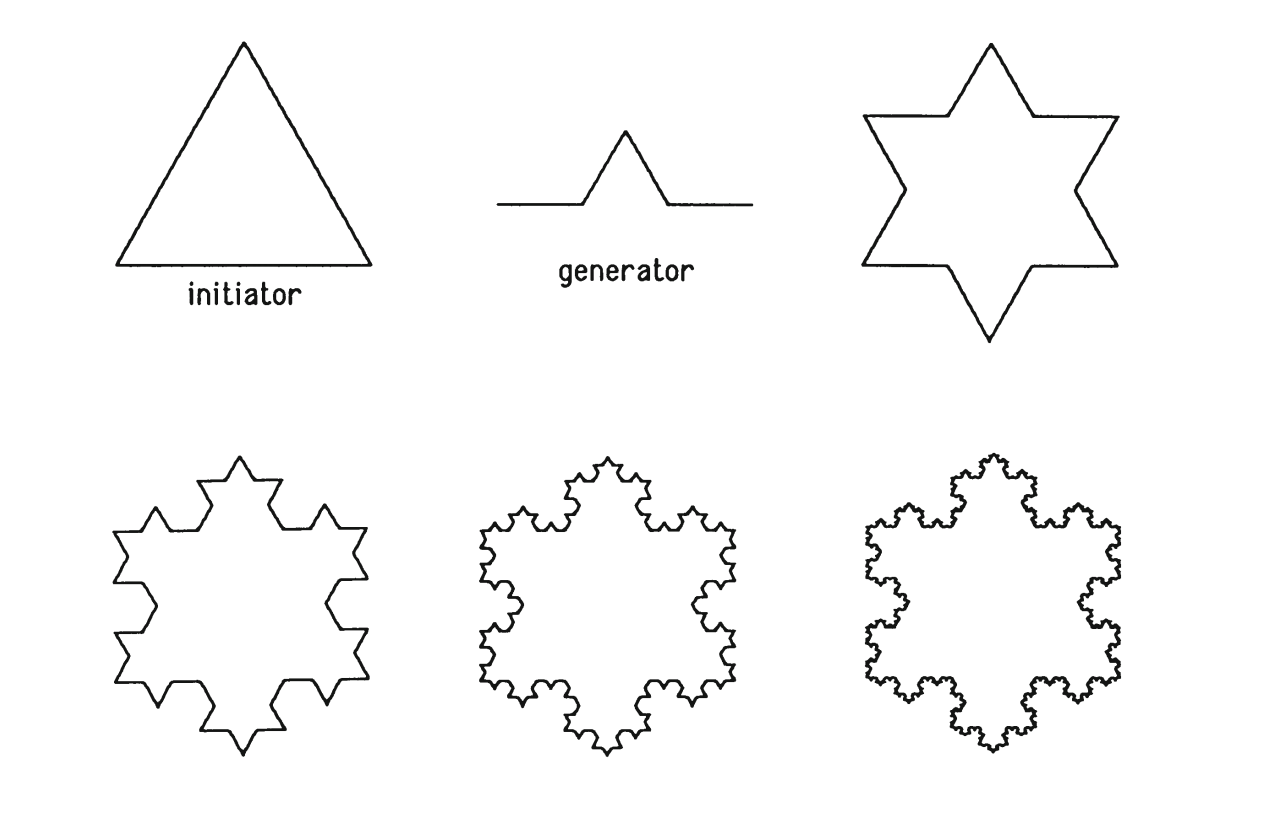
\includegraphics[scale=0.3]{Diagrams/snowflakeCurve.png}
		}
		\caption{Construction of the snowflake curve\cite{prusinkiewicz2013lindenmayer}.} \label{snowflake curve}
	}
\end{figure}
\FloatBarrier

\noindent
The snowflake curve starts with two parts, the initiator and the generator. The initiator is is the initial set of edges forming a certain shape, whereas the generator is a set of edges which can be used to replace each edge of the initiator to form a new shape. That new shape then becomes the initiator for the next generation, where each edge is again replaced by the generator. The result is a complex shape similar to that of a snowflake. The initiator, generator concept is a graphical representation of how rewriting systems operate, rather than the initiator and generator being a set of edges they are instead represented by a set of symbols or strings.

\section{Introduction to Formal Grammars}

In the context of computer science, grammars are defined as a set of rules governing which strings are valid or allowable in a language or text. They consist of syntax, morphology and semantics. Formal languages have been defined in the form of grammars to suit particular problem domains. It is natural for humans to communicate a problem or solution in the form of language, it is therefore intuitive to use a language to describe the desired outcome when dealing with the procedural generation of plant-life. In the past, formal grammars have been used extensively in computer science in the form of programming languages in which humans can provide a computer with a set of instructions to carry out in order to gain an expected result. The challenge is therefore to create a  grammar in the form of a rewriting system that facilitates the procedural generation of plant-life. A rewriting system such as the L-system operates in a way that is consistant with a context-free class of Chomsky grammar \cite{chomsky1956three}, similar to that of the programming language ALGOL-60 introduced by Backus and Naur in  1960\cite{backus1960report}. In figure \ref{chomsky grammars} below, there are two types of L-system grammars that overlap the classes of chomsky grammars, the OL-system and the 1L-system. The details of these two systems will be discussed in detail chapter \ref{l-system chapter}, but in summary, 0L-systems are grammars that can represent a context-sensitive Chomsky grammar but generally tend to be context-free, the main difference between the 0L-system and the 1L-system is that 1L-systems can be recursively enumerable. Furthermore, it is possible for a 1L-system to represent any 0L-system, therefore, 1L-system languages tend to be more complex and verbose when compared to 0L-systems, this creates a trade off between a more powerful and complex language or a less powerful but simpler language. 

\begin{figure}[htbp]
	{\centering
		\setlength{\fboxrule}{1pt}
		\vspace{7px}
		\fbox{
			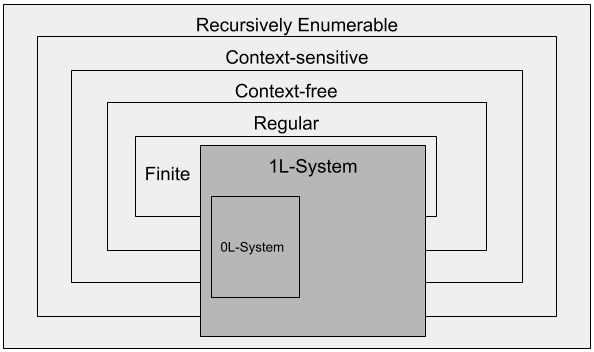
\includegraphics[scale=0.5]{Diagrams/ChomskyGrammar.png}
		}
		\caption{Diagram of the Chomsky hierarchy grammars with relation to the 0L and 1L systems generated by L-systems.} \label{chomsky grammars}
	}
\end{figure}
\FloatBarrier

\section{Structure of Thesis}

This thesis is split into three major parts. Part 1 focuses on the L-system itself, it defines the various types of L-systems for modeling plant-life, the concept of a parametric L-system as well as some techniques for definiting randomness and stochasticisity within an L-system in order to create variaty. Part 2 talks about the L-system rewriter implementation, covering how the L-system generates the resulting string and structures relavant rendering. Part 3 focuses on the interpretation and renderer implementation and how to render a convincing model of a tree on the screen, as well as simulation and animation of the generated plants.







\chapter{Lindenmayer Systems}  \label{l-system chapter} 
\begin{flushleft}

Aristid Lindenmayer is a well known biologist who started work on what would become known as the Lindenmayer System or L-system for short. Lindenmayer initially intended the L-systems to be to be used as a way to describe the development of simple organisms such as algae and bactaria. More recently the concept has been adapted to be used to describe larger organisms such as plants and trees. L-systems have also been used to describe non organic structures like music. \cite{worth2005growing} \\

\vspace{5mm}

An L-system at its core is a formal grammar made up of an \textit{alphabet} of symbols which are put together into strings, a set of rules is used to determine whether or not a symbol in the string should be rewritten with another symbol or string. What we end up with is a string of symbols which we can refer to as a set of states, for each state the rules determine what symbols to rewrite and what they should be replaced with or if they should be replaced at all.\\

\vspace{5mm}


In section \ref{Simple DOL-systems} below, I will be going into detail about a simple type of L-system called a Deterministic 0L-system.  D0L-systems serve as a good way to introduce the concept of an L-system.

\end{flushleft}

\section{Simple DOL-system} \label{Simple DOL-systems}

\begin{flushleft}

According to Prusinkiewicz and Hanan a simple type of L-systems are those known as deterministic 0L systems, where the string refers to the sequence of cellular states and the term '0L system' abbreviates 'Lindenmayer system with zero-sided interactions'.  With D0L systems there are only three major parts. There is a set of symbols known as the (\textit{alphabet}), the starting string or (\textit{axiom}) and the state transition rules (\textit{rules}). The alphabet is a set of states. The starting string or \textit{axiom} is the starting point containing one or more states. The transition rules dictate whether a state should remain the same or transition into a different state, remain the same or even disappear. \cite{prusinkiewicz2013lindenmayer}. \\

\vspace{5mm}

Below is an example of a deterministic 0L system: \\

\vspace{5mm}

We are given the \textit{alphabet} with symbols: A, B \\ 
The \textit{axiom}: A \\
The \textit{rule} set: \\ 
A $\rightarrow$ AB \\
B $\rightarrow$ A \\

\vspace{5mm}

The symbol $\rightarrow$ can be verbalised as "replaced by". Therefore the first rule is said to be, string 'A' is replaced by string 'AB' and the second rule is said to be 'B' is replaced by the string 'A'.\\
To start we take the first state in the \textit{axiom} which, in this case is the symbol 'A', we then check it against the first rule which is 'A', if the current state matches the rule state we replace 'A' with whatever the rules successor is, which is 'AB'. We would then move onto the next state in the axiom, however there is only one state in the axiom, 'A' so we are finished with the first generation. The states 'AB' then becomes the new starting string for the first generation. We can then continue by matching the rules once again to the new starting string. Below I have shown the string for each generation up to the sixth generation.\\

\vspace{5mm}

0.) A \\
1.) AB \\
2.) ABA \\
3.) ABAAB \\
4.) ABAABABA \\
5.) ABAABABAABAAB \\

\vspace{5mm}

This rewriting of strings using a set of rules is ultimately the underlying concept behind L-systems. There are a number of improvements that can be made to this type of L-system in order to accommodate for more complex and intricate structures. I will be talking about these in more detail in the following sections, however some important imporovements are: constants, variables, branching constructs, parametric l-systems, conditional rules and random values. //

\vspace{5mm}

An example of how an L-system can represent a real life biological structure would be Prusinkiewicz and Lindenmayer's simulation of a blue-green bacteria known as \textit{Anabaena catenula}\\

\vspace{5mm}

Prusinkiewicz and Lindenmayer created the following DOL-system representation shown below in the following grammar: \\

\vspace{5mm}

$w$ : $ a\textsubscript{r} $\\
\textit{p1} : $ a\textsubscript{r} $ $\rightarrow$ $a\textsubscript{l}b\textsubscript{r}$ \\
\textit{p2} : $ a\textsubscript{l} $ $\rightarrow$ $b\textsubscript{l}a\textsubscript{r}$ \\
\textit{p3} : $ b\textsubscript{r} $ $\rightarrow$ $a\textsubscript{r}$ \\
\textit{p4} : $ b\textsubscript{l} $ $\rightarrow$ $a\textsubscript{l}$ \\

\vspace{5mm}

The value $w$ is there to specify the axiom which is this case has the value of $ a\textsubscript{r} $. \textit{p1}, \textit{p2}, \textit{p3}, \textit{p4} are the names of the rules that follow after the semi-colon. In order to simulate Anabaena catenula we need four rules. \\
According to Prusinkiewicz and Lindenmayer "Under a microscope, the filaments appear as a sequence of cylinders of various lengths, with $a$-type cells longer than $b$-type cells. And the subscript $l$ and $r$ indicate cell polarity, specifying the positions in which daughter cells of type $a$ and $b$ will be produced. \cite{prusinkiewicz2012algorithmic} \\

\vspace{5mm}

The first five generations can be written as follows: \\

\vspace{5mm}

0.) $a_r$ \\
1.) $a_l b_r$ \\
2.) $b_l a_r a_r$ \\
3.) $a_l a_l b_r a_l b_r$ \\
4.) $b_l a_r b_l a_r a_r b_l a_r a_r$ \\
5.) $a_l a_l b_r a_l a_l b_r a_l b_r a_l a_l b_r a_l b_r$ \\

\vspace{5mm}



\end{flushleft}

\section{Constants and Variables}

\begin{flushleft}

Constants are symbols or states which don't have any significant value during the rewriting process and therefore will remain the same between generations however they do have significance when the final string is being interpreted and furthermore represented. There are a number of constants that have a fixed meaning when interpreted and are therefore known as commands. These values are:

\vspace{5mm}

$\bullet$ F: 				\hspace{10mm}  		Move forward by a specified distance whilst drawing a line \\
$\bullet$ f: 				\hspace{10mm} 		Move forward by a specified distance without drawing a line \\
$\bullet$ +: 				\hspace{10mm} 		Yaw to the right specified angle. \\
$\bullet$ -: 				\hspace{10mm} 		Yaw to the left by a specified angle.  \\
$\bullet$ /: 				\hspace{10mm} 		Pitch up by specified angle. \\
$\bullet$ $\backslash$: 	\hspace{10mm} 		Pitch down by a specified angle.  \\
$\bullet$ $\hat{}$: 		\hspace{10mm} 		Roll to the right specified angle. \\
$\bullet$ \&:				\hspace{10mm}  		Roll to the left by a specified angle.  \\

\vspace{5mm}

The question then remains why should they be interpreted using these commands and how are these instructions actually interpreted. As with any grammar, there is a number of ways of interpreting the string that is generated. One method proposed by Przemyslaw Prusinkiewics is "to generate a string of symbols using an L-system, and to interpret this string as a sequence of commands which control a 'turtle'" \cite{prusinkiewicz1986graphical}.\\

\vspace{5mm}

When talking about a turtle, prusinkiewicz is refering to turtle graphics. Turtle graphics is a type of vector graphics that can be carried out with instructions. It is named a turtle after one of the main features of the Logo programming language. The simple set of turtle instructions shown below, can be expressed in the form below and displayed as figure \ref{basic turtle}\\

\vspace{5mm}

1. Move forward by 1.\\
2. Rotate right by 90 degrees.\\
3. Move forward by 1.\\
4. Rotate left by 90 degrees \\
5. Move forward by 1. \\
6. Rotate left by 90 degrees. \\
7. Move forward by 1. \\
8. Rotate right by 90 degrees. \\
9. Move forward by 1.\\

\vspace{5mm}

\begin{figure}[htbp]
	{\centering
		\vspace{7px}
		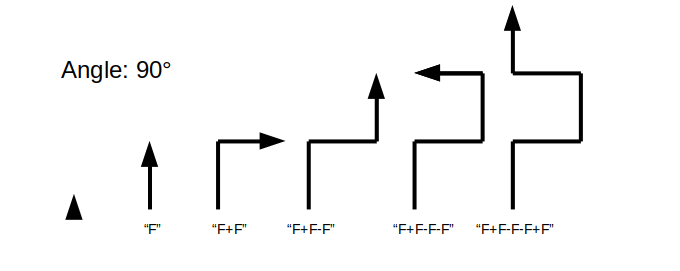
\includegraphics[scale=0.5]{Diagrams/basic_turtle.png}
		\caption{Diagram showing a turtle interpreting simple L-system string.} \label{basic turtle}
	}
\end{figure}
\FloatBarrier

\vspace{5mm}

There are a further two commands which I will be covering in detail in section \ref{branching}. We can also have constant numerical values that can be used. For instance we could pass in a constant value of 1.0 as a parameter to the forward instruction as follows.

\vspace{5mm}

F(1.0)+F(1.0)-F(1.0)+F(1.0)

\vspace{5mm}

In doing this, we are able to specify that we would like to move forward by a specified amount. In this case we would like to move forward by 1.0 unit length. We will be covering parametric L-systems in great detail in section \ref{parametric}.

\end{flushleft}

\section{Branching} \label{branching}

\begin{flushleft}

In the previous section there are two turtle commands in particular which were  not covered. These are the square bracket commands "[", "]". The square bracket characters instruct the turtle object to save its position and rotation for the purpose of being able to restore that saved position and rotation later on. This allows the turtle to jump back to a previous position, facing the same direction as it was before. We can then branch off in a different direction.\\

\vspace{5mm}

A way to keep track of these saved locations, is in the form of a stack structure. Each time the "[" is called the current position and orientation of the turtle is saved to the top of the stack. While conversely when the "]" is called we restore the turtles position back to whatever position and orientation is stored on the top of the stack. \\

\vspace{5mm}

An example of this can be shown below in figure 2.2.\\

\begin{figure}[htbp]
	{\centering
		\vspace{7px}
		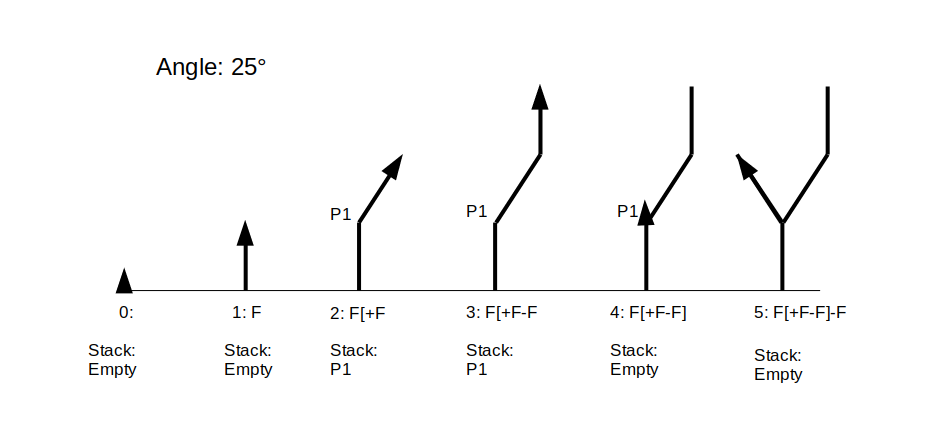
\includegraphics[scale=0.5]{Diagrams/branching_turtle.png}
		\caption{Diagram showing a turtle interpreting an L-system incorporating branching.}
	}
\end{figure}
\FloatBarrier

\end{flushleft}

\section{Parametric L-system} \label{parametric}

With simplistic L-systems like the algae representation above, there are a number of details that are skipped over when making this simplistic representation. (talk about the representation for both parameterized and non parameterised Algae systems). When it comes to representing trees as L-systems a simplistic approach would be to just assume that the width and length of each branch section is constant and will not vary depending on where in the tree it is. We can also assume that the angles at which a branch may split is also constant, say 25 degrees. 
The resulting representation of this L-system is a tree like structure, however it is not a very accurate representation of a real tree in nature. \\
In order to more accurately model trees we need to take into account the branch width, height, branching angles. There are two different approaches to solving this added complexity. One would be to increase the complexity of the L-system grammar and the other would be to increase the complexity of the interpretation of the L-system. \\
For instance defining an complex L-system grammar with a less complex interpreting system can give a huge amount of flexibility to define parameters that can accurately define exactly how the L-system should be interpreted, and because the complexity is with the L-system rewriting you also have the control of being able to change the L-system rules. \\
\\ 
A parametric l-system be represented as the following: \\
\\
\hspace*{3cm} n = 8\\
\\
\hspace*{3cm} R 1.456\\
\hspace*{3cm} r1 85\\
\hspace*{3cm} wr 0.707\\
\\
\hspace*{3cm} w : A(5)\\
\\
\hspace*{3cm} p1 : A(w) : * : F(1)!(w)[/(r1)A(w*wr)][$\backslash$(r1)A(w*wr)]\\
\hspace*{3cm} p2 : F(s) : * : F(s*R)\\
\\
The above l-system gives the resulting representation shown below in figure 3.8. 

\begin{figure}[htbp]
	{\centering
		\vspace{7px}
		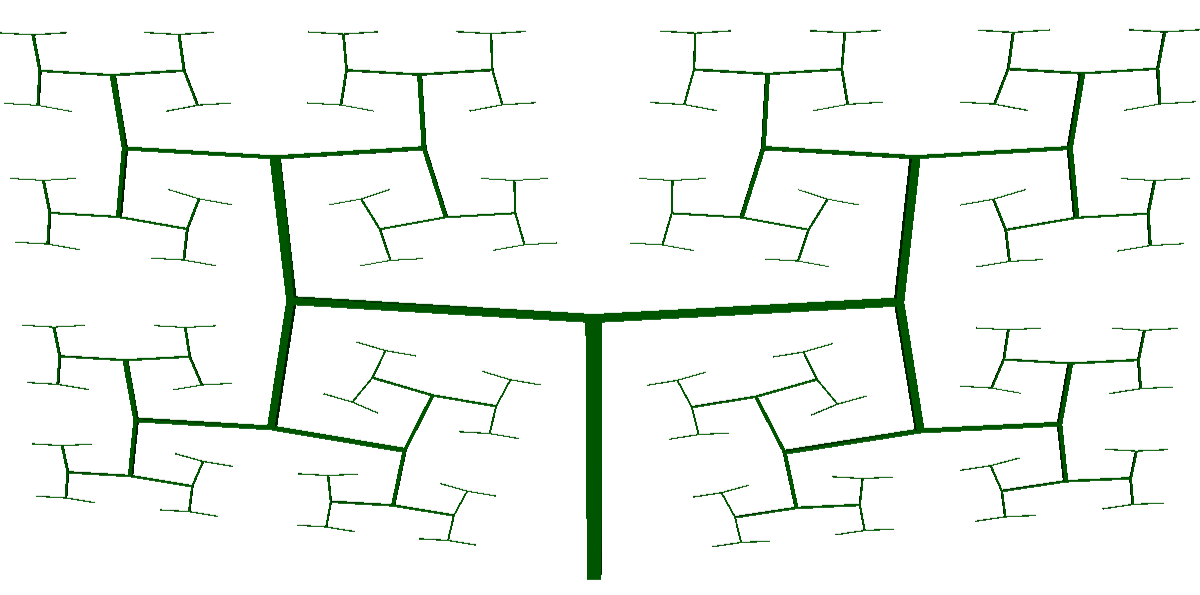
\includegraphics[scale=0.20]{ParametricLsystem/branchingPattern.png}
		\caption{3D Parametric L-system.}
	}
\end{figure}

Similarly to the 2D L-system in section \ref{Simple DOL-systems}, n refers to the number of iterations that we would like to rewrite the L-system. w refers to the Axiom string, the \#define R 1.456 states that there is a constant number that will be used somewhere in the production rules, with the name R and the value 1.456. P1, P2 refer to the production rules. The 3D L-system introduces the concept of a module.\\
A module is an instruction or variable which has zero or more parameters. The Axiom A(5) is a module with one parameter which is the number 5. A parameter can either be a number, variable or even an expression of variables and numbers. For instance A(a + 1, a * b) is a valid module A with two parameters a + 1 and a * b, where a and b are variables, however this is only a valid module if the value of a and b can be determined. Each module is treated as a single instruction, it will either be overwritten when matched with a production rule or the expression of each parameter is evaluated and is left unchaged for use when interpretted.\\
Each production rule is made up of four parts the name, the predecessor module, the condition and the successor modules, each part is separated by a colon. Therefor the predecessor for p1 is A(w), the condition is a '*' which means that in this case there are no conditions, and the successor is F(1)!(w)[/(r1)A(w*wr)][$\backslash$(r1)A(w*wr)]\\
\\
Initially we iterate through the Axiom modules and compare them to the production rule. A match is determined if they meet three criteria.\\
\\
$\bullet$ The name of the axiom module matches the name of the production predecessor. \\
$\bullet$ The number of parameters for the axiom module is the same as the number of parameters for the production predecessor. \\
$\bullet$ The condition of the production evaluates to true. If there is no condition then the result is true by default.\\
\\










\chapter{3D Mathematics}
\section{The Use of L-systems in 3D applications}

L-systems have been talked about and researched since its inception in 1968 by Aristid Lindenmayer. Over the years it's usefulness in modelling different types of plant life has been very clear, however its presence has been quite absent from any mainstream game engines for the most part, these engines relying either on digital artists skill to develop individual plants or on 3rd party software such as SpeedTree. These types of software use a multitude of different techniques however their methods are heavily rooted in Lindenmayer Systems. 

\section{L-system grammars}

According to Prusinkiewicz and Hanan a simple type of L-systems are those known as deterministic 0L systems, where the string refers to the sequence of cellular states and '0L system' abbreviating 'Lindenmayer system with zero-sided interactions'.  With 0L systems there are only three major parts. There is a set of symbols (\textit{alphabet}), the starting string (\textit{Axiom}) and state transition rules (\textit{rules}). The alphabet is a set of states. The starting string is a starting point containing one or more states. The transition rules are rules that dictate whether a state should remain the same or transition into a different state or even disappear. \cite{prusinkiewicz2013lindenmayer}. \\
\\
An example of a deterministic 0L system is that a simplified model for the growth of algae: \\
\\
We are given the \textit{alphabet}: A, B \\ 
and the \textit{axiom}: A \\
and the \textit{rule} set: \\ 
A $\rightarrow$ AB \\
B $\rightarrow$ A \\
\\
If we then apply the rules to the L-system we find it creates the following generation structure. \\
1.) A \\
2.) AB \\
3.) ABA \\
4.) ABAAB \\
5.) ABAABABA \\
6.) ABAABABAABAAB \\
\\
This rewriting of initial string using a set of rules is ultimately the underlying concept behind L-systems. There are a number of improvements that can be made to this type of L-system in order to accommodate for more complex and intricate structure. One of which is the inclusion of \textit{constants}. Constants can be considered any state that does not have a rule associated with it or remains the same from generation to generation and therefore holds a consistent value or meaning. Some examples of constants are stated below. \\
\\
$\bullet$ +: Rotate to the right specified angle. \\
$\bullet$ -: Rotate to the left by a specified angle.  \\
$\bullet$ [: Save the current position and angle. \\
$\bullet$ ]: Load a saved position and angle. \\
\\
These types of constants are useful when we are dealing with fractal structures.

\section{Basic 2D L-systems} 

There are a number of fractal geometry that have become well known particularly with regards to how they can seemingly imitate nature \cite{mandelbrot1982fractal}. Particularly with the geometry such as the Koch snowflake which can be represented using the following L-system.

\begin{figure}[htbp]
	\raggedright
	\textbf{\underline{Koch Curve:}} \\
	\textbf{Alphabet:} F \\
	\textbf{Constants:} +, - \\
	\textbf{Axiom:} F \\
	\textbf{Angle:} 90$^\circ$ \\
	\textbf{Rules:} \\
	F $\rightarrow$ F+F--F+F\\
	{\centering
		\vspace{7px}
		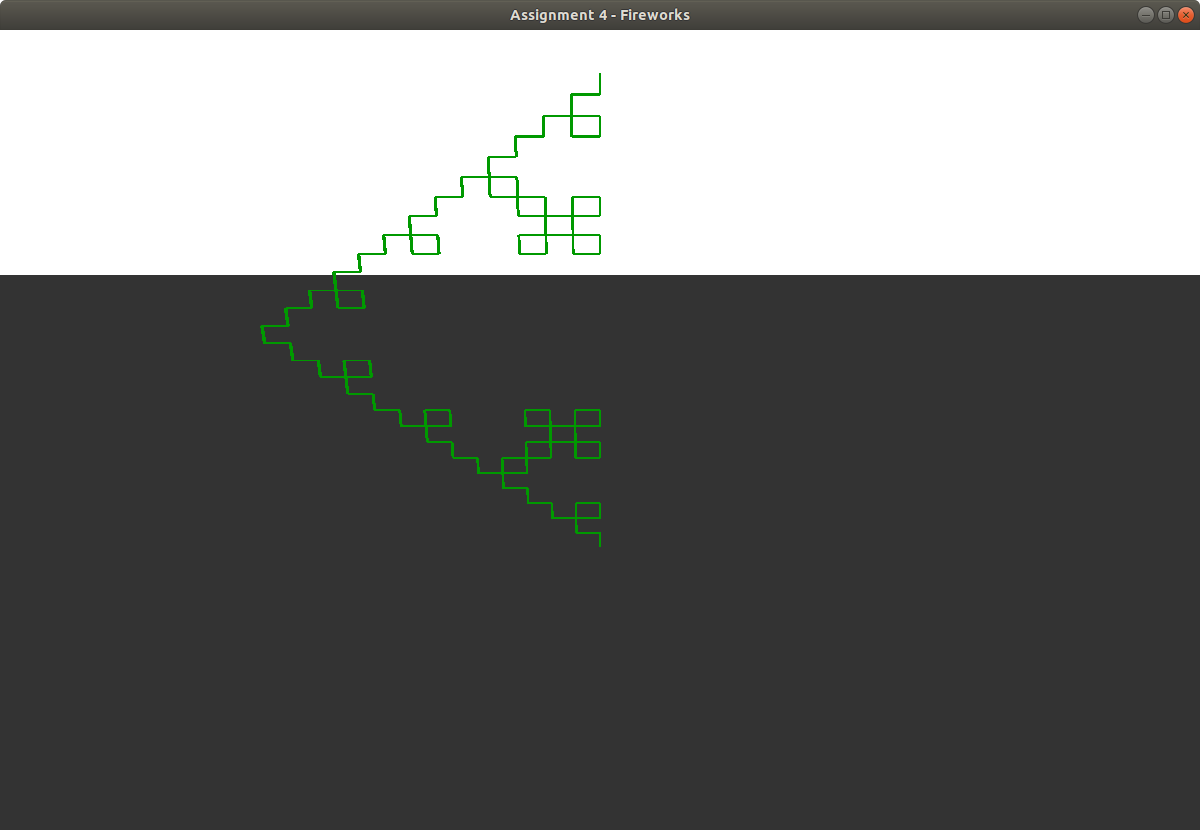
\includegraphics[scale=0.8]{KochCurve/KochCurve04.png}
		\caption{Koch Curve.}
	}
\end{figure}
\begin{figure}[htbp]
	\raggedright
	\textbf{\underline{Sierpinski Triangle:}} \\
	\textbf{Alphabet:} A, B \\
	\textbf{Constants:} +, - \\
	\textbf{Axiom:} A \\
	\textbf{Angle:} 60$^\circ$ \\
	\textbf{Rules:} \\
	A $\rightarrow$  B-A-B \\
	B $\rightarrow$ A+B+A\\
	{\centering
		\vspace{7px}
		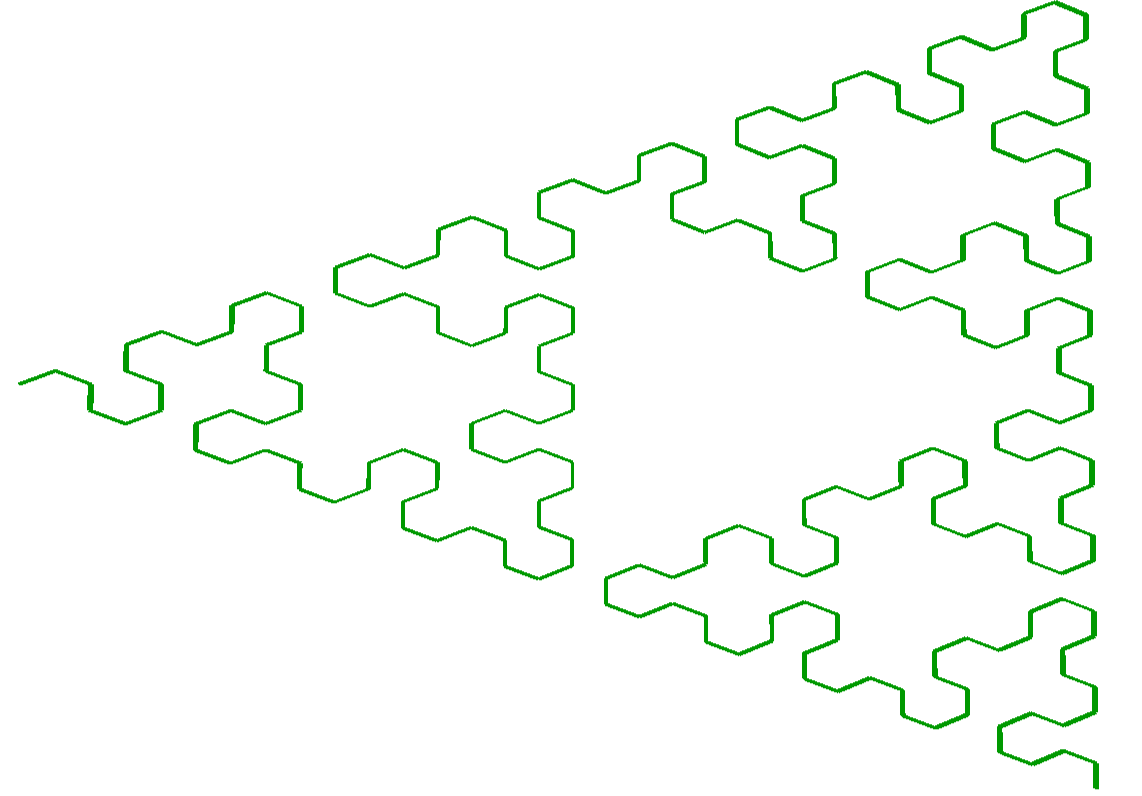
\includegraphics[scale=0.17]{SierpinskiTriangle/SierpinskiTriangle06.png}
		\caption{Sierpinski Triangle.}
	}
\end{figure}
\begin{figure}[htbp]
	\raggedright
	\textbf{\underline{Dragon Curve:}} \\
	\textbf{Alphabet:} F, X, Y \\
	\textbf{Constants:} +, - \\
	\textbf{Axiom:} FX \\
	\textbf{Angle:} 90$^\circ$ \\
	\textbf{Rules:} \\
	X $\rightarrow$ X+YF+ \\
	Y $\rightarrow$ -FX-Y\\
	{\centering
		\vspace{7px}
		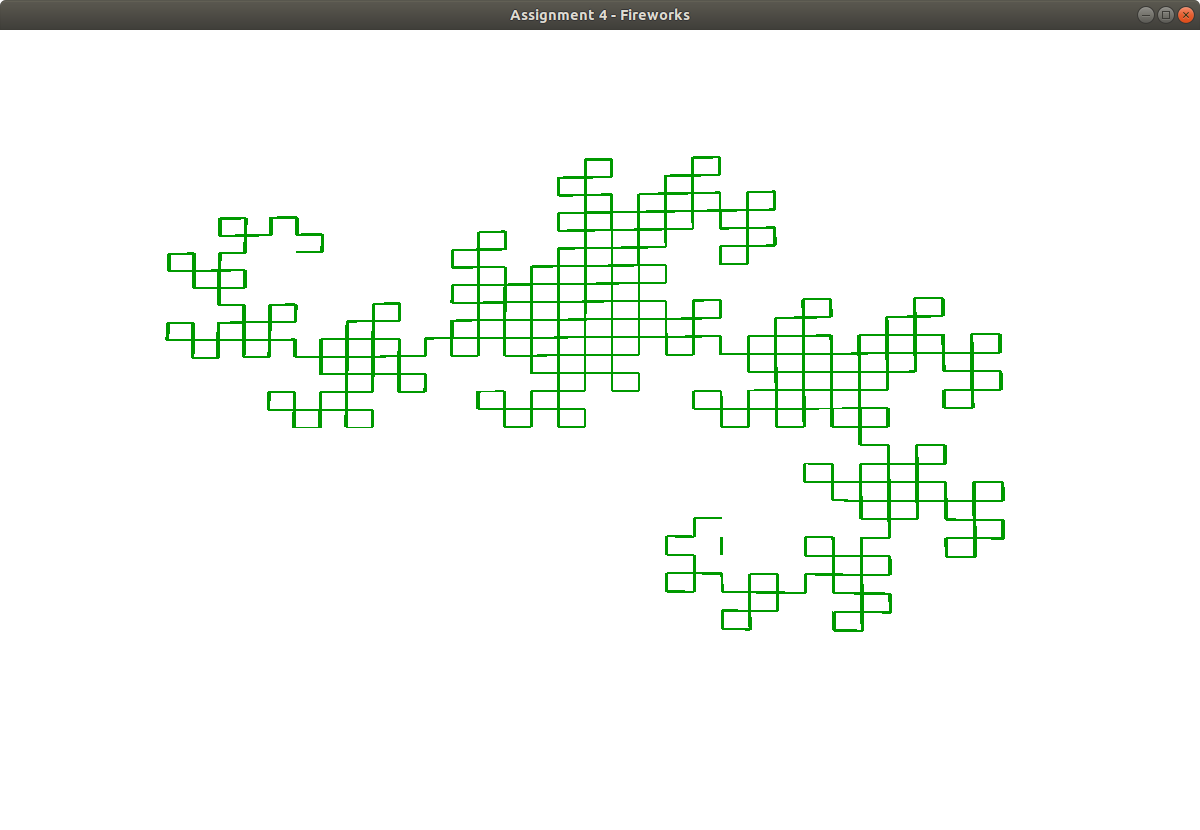
\includegraphics[scale=0.17]{DragonCurve/DragonCurve10.png}
		\caption{Dragon Curve.}
	}
\end{figure}
\begin{figure}[htbp]
	\raggedright
	\textbf{\underline{Fractal Plant:}} \\
	\textbf{Alphabet:} X, F\\
	\textbf{Constants:} +, -, [, ] \\
	\textbf{Axiom:} X \\
	\textbf{Angle:} 25$^\circ$ \\
	\textbf{Rules:} \\
	X $\rightarrow$ F-[[X]+X]+F[+FX]-X\\
	F $\rightarrow$ FF \\
	{\centering
		\vspace{7px}
		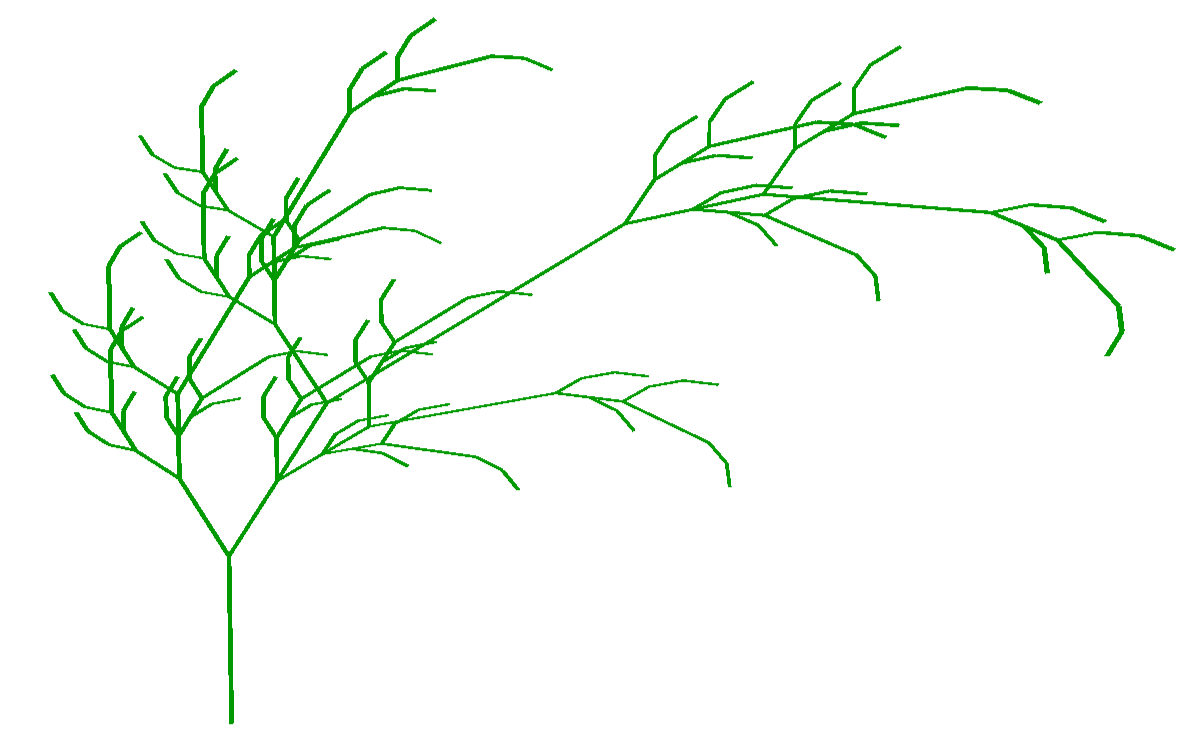
\includegraphics[scale=0.15]{FractalPlant/FractalPlant05.png}
		\caption{Fractal Plant.}
	}
\end{figure}
\begin{figure}[htbp]
	\raggedright
	\textbf{\underline{Fractal Bush:}} \\
	\textbf{Alphabet:} F\\
	\textbf{Constants:} +, -, [, ] \\
	\textbf{Axiom:} F \\
	\textbf{Angle:} 25$^\circ$ \\
	\textbf{Rules:} \\
	F $\rightarrow$ FF+[+F-F-F]-[-F+F+F]\\
	{\centering
		\vspace{7px}
		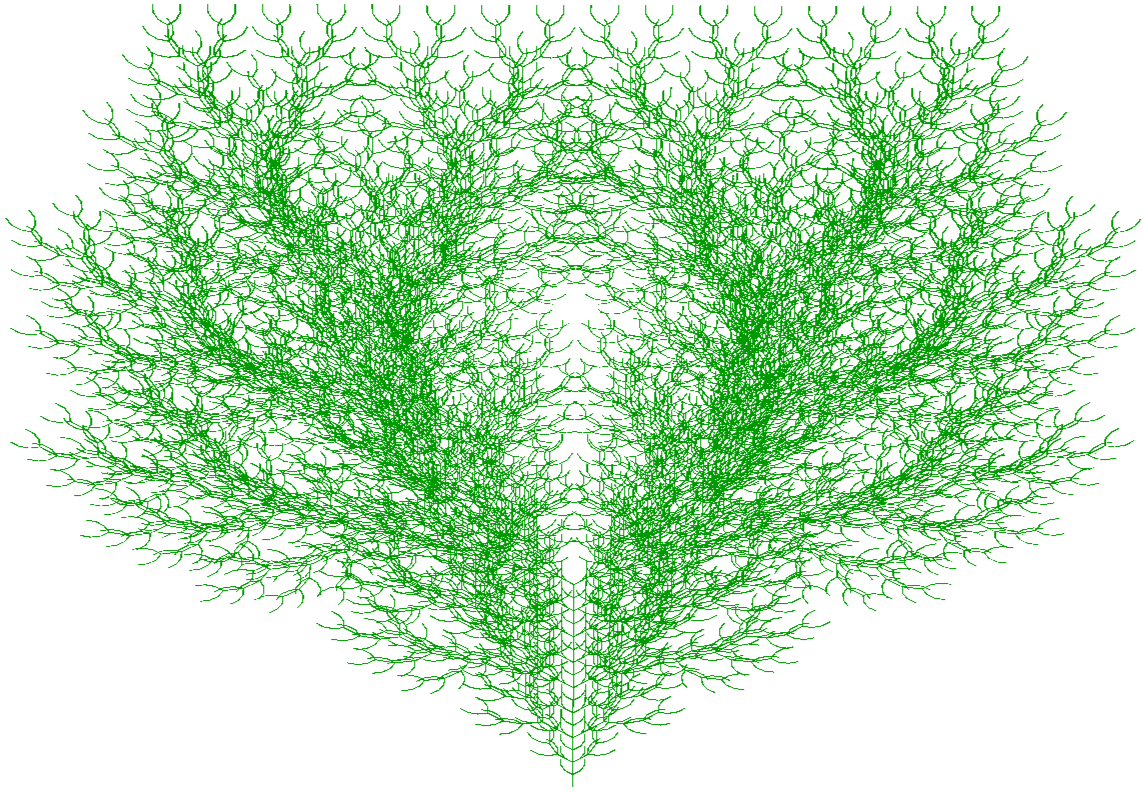
\includegraphics[scale=0.15]{FractalBush/FractalBush06.png}
		\caption{Fractal Bush.}
	}
\end{figure}

\FloatBarrier
\newpage
\section{Branching Filaments}

\chapter{L-system Rewriter Implementation}
\section{Motion Equations}

Torque\\
$ \tau = I\alpha $ \\
$ \tau = f \otimes R $ \\
\\
Mass \\
$ M = \Pi~ r ^ 2 h $ 

Inertia\\
$ I = \frac{1}{3} M L ^ 2 $ \\ 
\\
Angular Acceleration\\
\\
$ \omega = \omega _0 \alpha t $ \\
\\
Next angle equation\\
$ \theta = \theta _0 + \omega _0 t + \frac{1}{2} \alpha t ^2 $ \\
\\

\section{Hook's Law}

$ f = -k _s x $\\
$ f = -k _s x + k _d v $\\

\chapter{Physics Simulation}

\lettrine[lines=3]{T}{}he string interpreter is one of the major components of plant generation and it is the final step in the process of procedural generation. The output of this stage of processing is dependant on what the L-system is representing, in this case it is responsible for interpreting the resulting string of modules provided by the L-system rewriter, and uses this to generate the 3D models, structures and data of the resulting plant, which is then rendered and simulated on the screen using the OpenGL framework. The generation of plant-life has three main stages, the first part consists of a turtle graphics interpreter which takes the string of modules as a set of instructions, it starts from the root of the tree and generates a skeleton made up of joints, this is similar to the techniques used in skeletal rigging in animation \cite{gregory2014game}. The joints within the tree skeleton each represents a branch segment which has some information about the properties of that segment. These segements can be used to generate the vertex, index and other data that make up the 3D models of the plant. These models can finally be passed to the final part of string interpreter which is the renderer, the renderer is reponsible for taking all the vertices, indices, textures and shaders and organising it in an optimal way that enables rendering the plant on the screen, as well as the physical simulation of the tree skeleton. The stages of string interpretation can be seen in figure \ref{l-system interpreter} below. 

\begin{figure}[htbp]
	{\centering
		\vspace{7px}
		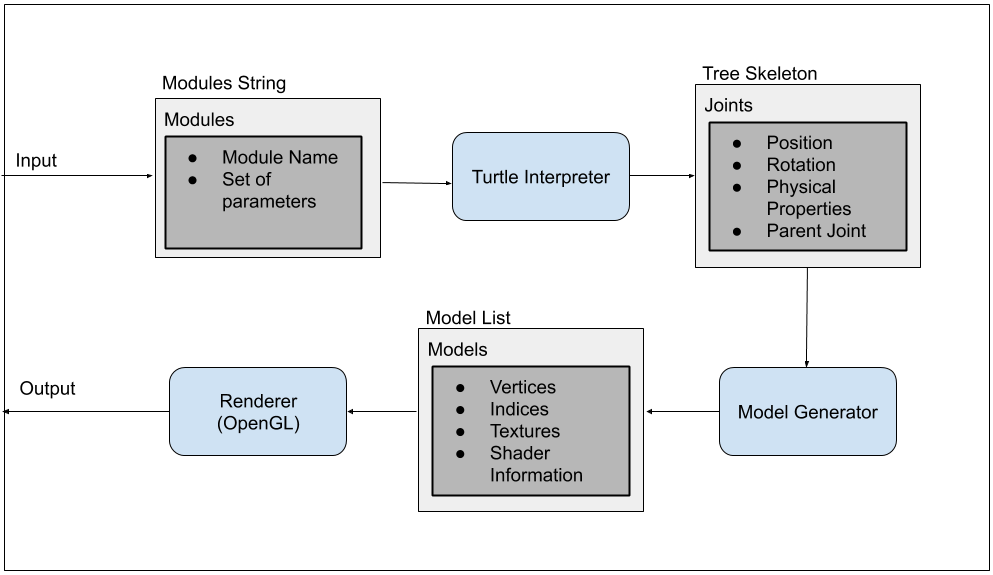
\includegraphics[scale=0.4]{Diagrams/L-systemInterpreter.png}
		\caption{Diagram of the stages of L-system interpretation and rendering} \label{l-system interpreter}
	}
\end{figure}
\FloatBarrier

\noindent
This chapter will cover each stage of the string interpreter implementation in detail, as well as well as talk about how the interpreter is able to simulate and animation the plants movements under forces such as gravity and wind in real time. 

\section{Turtle Graphics Interpreter}

The main purpose of the turtle graphics interpreter is to take the string of modules from the L-system rewriter, and interpret it as a list of turtle graphics instructions. As briefly covered in chapter \ref{l-system chapter}, each module name within the L-systems resultant string represents a particular meaning to the turtle graphics interpreter. The meaning of the module names are predefined in the string interpreter and are dependant on what the L-system is trying to represent. The L-system defined for this thesis is a parametric L-system, which allows each module to also provide a number of optional parameters. These may also carry a particular meaning for the interpreter. For instance the forward instruction or module name \say{F} can have three parameters. The value of the first parameter is the distance to move forward, this can also be seen as the length of the branch segment. The second and third parameter is the spring constant of the branch and the mass of the branch repectively. These give some information to the physics simulation in order to animate the plant. Below is a table describing the L-system module names as well as the parameter meanings for the turtle graphics interpreter.

\begin{table}[h!]
\centering
\begin{tabular}{ | c | l | l | l |}
\hline
	Instruction Name 	& Parameter 1 & Parameter 2 & Parameter 3 \\  
\hline
\hline
	F 							& Distance	& Spring Constant	& Branch Mass\\
\hline
	f 							& Distance	& Spring Constant	& Branch Mass\\
\hline
	+ 							& Angle of rotation &			&\\
\hline
	- 							& Angle	of rotation	&			&\\
\hline
	/ 							& Angle	of rotation	&			&\\
\hline
	$\backslash$ 				& Angle	of rotation	&			&\\
\hline
	$\land$ 					& Angle	of rotation	&			&\\
\hline
	\& 							& Angle	of rotation	&			&\\
\hline
	! 							& Branch width		&			&\\
\hline
\end{tabular}
\caption{Table of turtle instruction symbols and their meaning to the interpreter}
\label{instruction table 1}
\end{table}
\FloatBarrier

\noindent
Each modules instruction is carried out one by one to generate the plants skeletal structure, which is made up of joints. The joints hold information about the properties of each particular segement or object of the plant. The joints properties are the position, orientation, scale, parent joint as well as its physical characteristics. It is important to note that all of the scales and rotations must happen before the forward movement. As the rotations change the orientation of the brach and then the movement generates the joint itself. A joint is defined by the figure below:

\begin{figure}[htbp]
	{\centering
		\vspace{7px}
		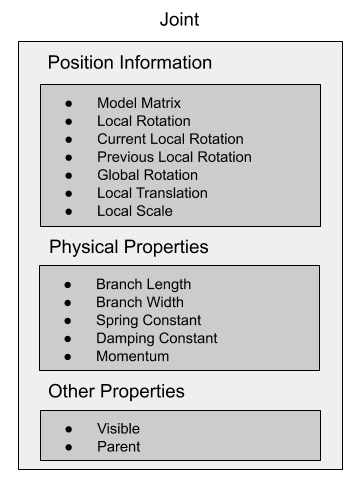
\includegraphics[scale=0.6]{Diagrams/JointDiagram.png}
		\caption{Diagram for the properties of a joint} \label{joint properties}
	}
\end{figure}
\FloatBarrier

\noindent
Figure \ref{joint properties} shows that there is in fact a large amount of information stored for the position and orientation of each joint. This is because the rotation of the joint is stored in both a local and global space. Local space refers to the rotation of the joint relative to its parent rotation, this is useful as it allows the manipulation of subsequent child joints, whilst leaving other joints local rotation unchanged. Global space, also known as world space, is the rotation of each joint relative to the world itself this is useful for understanding the current rotation of the joint relative to the world for instance calculating the torque or force calculations due to gravity. It is important to store both the current and previous rotations as they are used to calculate the rate of change for physics calculations.

The physical properties for each joint are the parts are what will affect model generation as well as physics simulations. These properties include the length, width, spring constant, damping constant as well as the current momentum of the branch. 

Take the following string of modules \say{F(1)[/(90)F(1)$\backslash$ (90)F(1)]-(90)F(1)+(90)F(1)}, the alphabet is made up of seven unique modules F, /, $\backslash$, [, ], + and -. According to the as discussed in previous chapters the \say{F} symbol represents a move forward, and \say{+}, \say{-}, \say{/}, \say{$\backslash$} symbolize different rotations, and the \say{[} and \say{]} represent save and load state respecively. The aforementioned symbols each have a single parameter except the load and save state. It is the turtle graphics interpreters job to understand what these parameters are and how to interpret them. In this case all of the \say{F} modules have the parameter value of 1, and all of the rotation modules have the parameter of 90. These are interpreted as the distance to move forward and the change in angle from the previous joint in degrees. This interpretation can be represented with the joint structure shown in figure \ref{skeleton diagram} below:

\begin{figure}[htbp]
	{\centering
		\vspace{7px}
		\setlength{\fboxrule}{1pt}
		\fbox{
			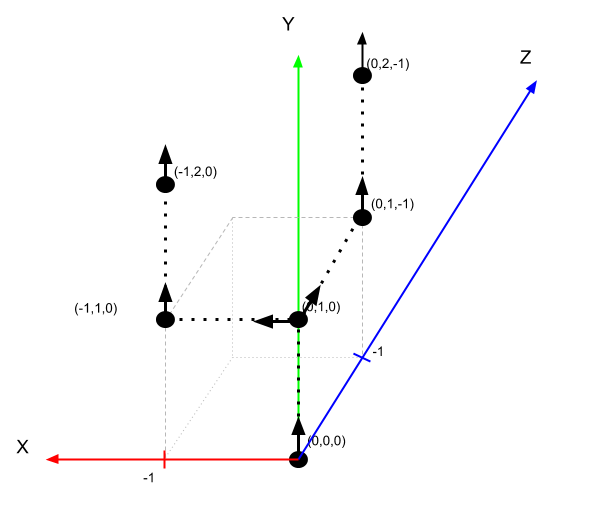
\includegraphics[scale=0.4]{Diagrams/SkeletonJoints.png}
		}
		\caption{Diagram of a simple plant skeleton with joint position and orientation.} \label{skeleton diagram}
	}
\end{figure}
\FloatBarrier


\section{3D Mathematics}

In any 3D application, mathematical models are used to represent the positions, rotations and scale of objects within a given scene. All objects within a 3D application are represented by a set of vertices or points, which can be represented with X, Y and Z coordinates. Three vertices can make up one triangle also called a face, multiple faces will then make up a whole 3D object. The use of mathematical methods in 3D graphics is to be able to manipulate all vertices of an object in a consistant way, thus rotating, translating or scaling the object within the scene. This section will provide sufficient background on some of most important concepts of 3D Mathematics, such as vectors, matrices and quaternions, which are widely used in the turtle graphics interpreter as well as the model generator.

\subsection{Vectors}

Vectors have many meanings in different contexts, in \acrshort{3d} computer graphics, often vectors are refering to the Euclidean vector. The Euclidean vector is a quantity in $n$-dimensional space that has both magnitude (the length from A to B) and direction (the direction to get from A to B). Vectors can be represented as a line segment pointing in a direction, with a certain length. A \acrshort{3d} vector can be written as a triple of scalar values eg: $(x, y, z)$

The most common operations on vectors are multiplication by a scalar, addition, subtraction, normalisation and the dot and cross product. The multiplication by a scalar value can be simply seen as scaling the magnitude of the vector itself, this can be done uniformly or non-uniformly as seen in the equation below:

\begin{equation}
a \otimes s = (a_x s_x, a_y s_y, a_z s_z)
\end{equation}

\noindent
Where $\otimes$ is the component-wise product of a vector $a$ and the scaling vector $s$. Similar to the scalar product of a vector the addition and subtraction of two vectors is the component-wise sum or difference. 

\begin{equation}
\begin{aligned}
a \oplus b = [(a_x + b_x), (a_y + b_y), (a_z + b_z)]\\
a \ominus b = [(a_x - b_x), (a_y - b_y), (a_z - b_z)]
\end{aligned}
\end{equation}

\begin{figure}[htbp]
	{\centering
		\setlength{\fboxrule}{1pt}
		\vspace{7px}
		\fbox{
			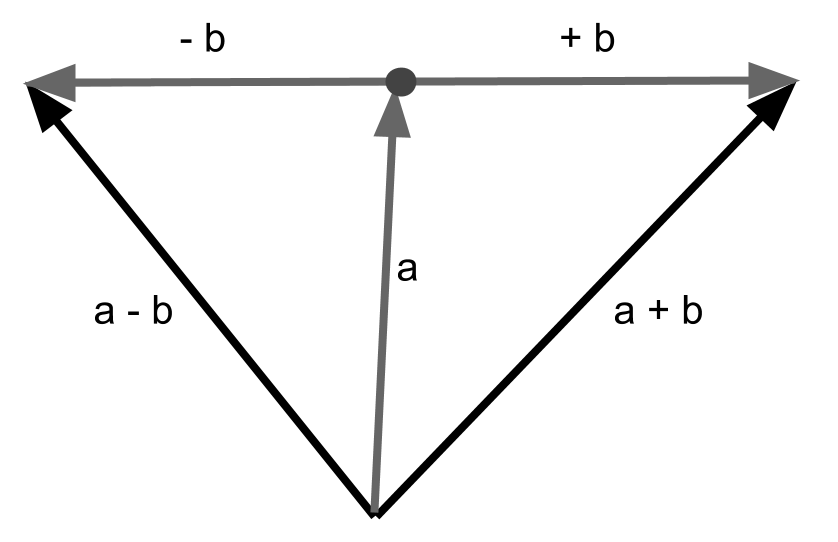
\includegraphics[scale=0.2]{Diagrams/vector_addition.png}
			\label{3DAxisFigure}
		}
		\caption{Table of common dot product tests between two vectors.}
	}
\end{figure}
\FloatBarrier

\noindent
A useful type of vector is known as a unit vector. This is a type of vector which has a magnitude of 1. Unit vectors are used extensively in computer graphics particularly with ragards to \gls{Shader}s. Take the vector v its magnitude $\alpha$ can be calculated by taking the square root of the product its components squared, as seen below 

\begin{equation}
	\alpha =~ \mid \textbf{v} \mid~ = \sqrt{\textbf{v}^2_x + \textbf{v}^2_y + \textbf{v}^2_z}
\end{equation}

The unit vector can then be calculated by taking the product of $v$ and the reciprocal of its magnitude shown in the following equation.

\begin{equation}
	\upsilon = \frac{\textbf{v}}{\alpha} = \frac{1}{\alpha} \textbf{v}
\end{equation}

There are many different ways to multiply vectors, however, in 3D graphics there two main multiplications. These being the dot and cross product. The dot product yields a scalar by adding the products of the vector product components. The cross product on the other hand is the product of two vectors which gives a vector which is perpendicular. The dot product can be calculated using the formula below: 

\begin{equation}
a \cdot b = a_x b_x + a_y b_y + a_z b_z = d
\end{equation}

\noindent
Some of the main uses for dot products within 3D graphics is to find whether two vectors are collinear, perpendicular, in the same direction or opposite directions. One possible use for this is to find the dot product of two branches directions in order to find out if they growing in the same direct or in opposite directions. In the table \ref{dot product test} below, there are each of the dot product test diagrams as well as the test equation where $ab = \mid a \mid \mid b \mid = a \cdot b$.

\begin{table}[h!]
\centering
\begin{tabular}{ | c | c | c |}
\hline
	Test 	& Equation & Example\\  
\hline
\hline
	Collinear 							& $(a \cdot b) = ab$ & 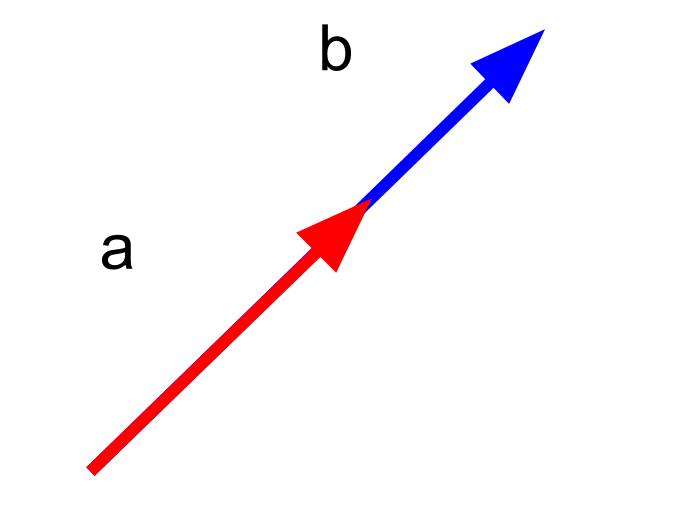
\includegraphics[scale=0.1]{Diagrams/vector1.png}\\
\hline
	Opposite Collinear 					& $(a \cdot b) = -ab$ &	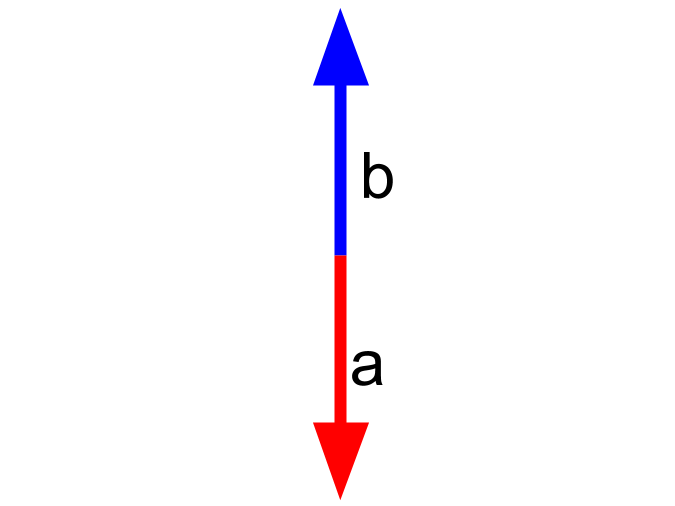
\includegraphics[scale=0.1]{Diagrams/vector2.png}\\
\hline
	Perpendicular 						& $(a \cdot b) = 0$	&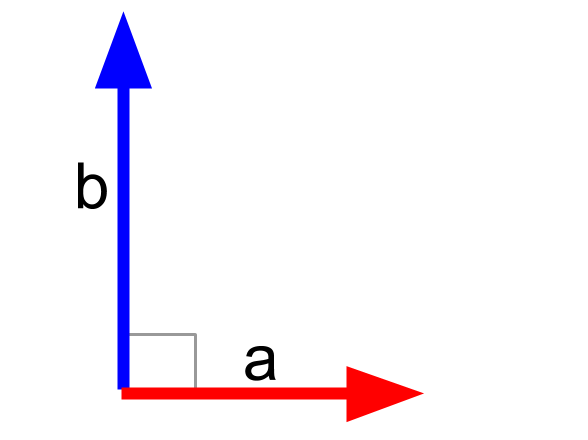
\includegraphics[scale=0.1]{Diagrams/vector3.png}\\
\hline
	Same Direction 						& $(a \cdot b) > 0$ &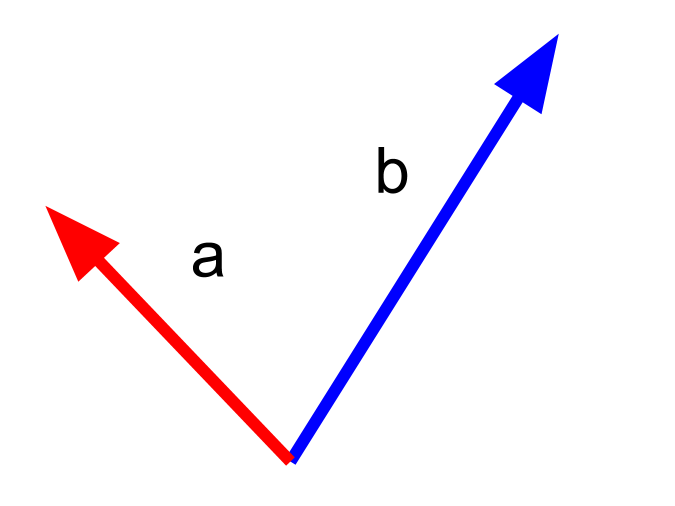
\includegraphics[scale=0.1]{Diagrams/vector4.png}\\
\hline
	Opposite Direction 					& $(a \cdot b) < 0$ &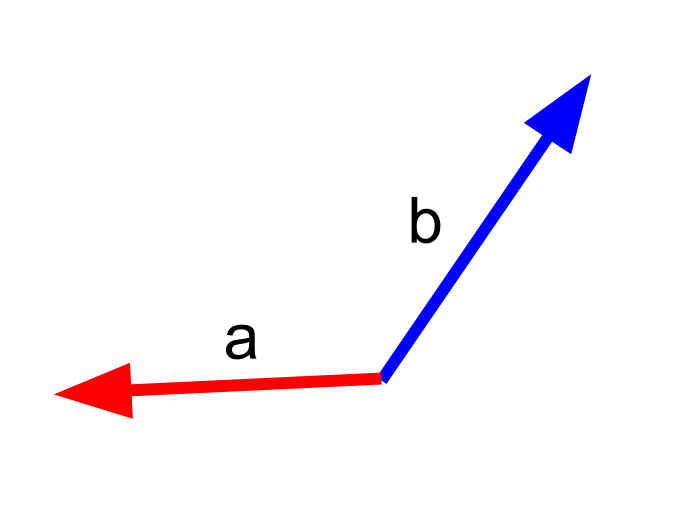
\includegraphics[scale=0.1]{Diagrams/vector5.png}\\
\hline

\end{tabular}
\caption{Table of turtle instruction symbols and their meaning to the interpreter}
\label{dot product test}
\end{table}
\FloatBarrier

\noindent
The cross product also known as the outer product takes two vectors and finds the perpendicular vector of the two vectors, this is only possible in 3D space and can be expressed in the following formula using the left-hand rule: 

\begin{equation}
a \times b = [(a_y b_z - a_z b_y), (a_z b_x - a_x b_z), (a_x b_y - a_y b_x)]
\end{equation}

\noindent
The result of a cross product can be seen in figure \ref{Cross product diagram} below. Where vectors $a$ and $b$ give the perpendicular vector $a \times b$. The cross product is very useful within physics calculations when it is necessary to find the rotational motion. 

\noindent
Some of the properties of the cross product are as follows:

\begin{itemize}
	\item is non-commutative, meaning order matters($a \times b \not= b \times a$).
	\item is anti-commutative ($a \times b = -(a \times b)$).
	\item is distributive with addition ($a \times (b + c) = (a \times b) + (a \times c)$).
\end{itemize}

\begin{figure}[htbp]
	{\centering
		\setlength{\fboxrule}{1pt}
		\vspace{7px}
		\fbox{
			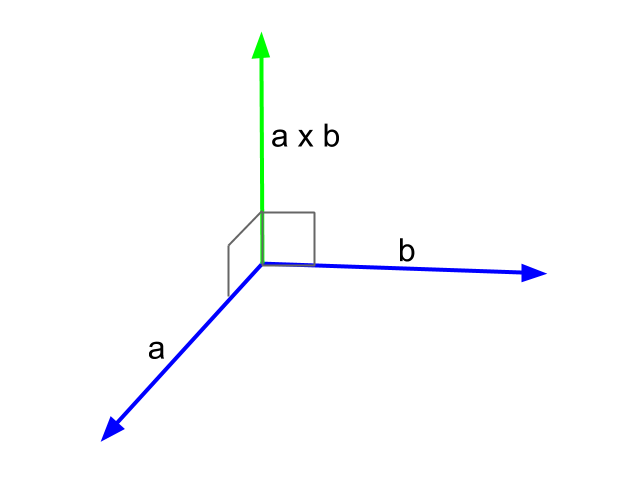
\includegraphics[scale=0.25]{Diagrams/cross_product.png}
			\label{Cross product diagram}
		}
		\caption{Diagram of the cross product of two vectors a and b.}
	}
\end{figure}
\FloatBarrier

\subsection{Matrices}

A model in 3D space will exist as a set of vertices which each have a position. Moving the model requires moving all of the the vertices of that model without distorting it in any way, this is called a model transform. There are four main types of transforms; translation, rotation, scale and shear. Matrices are a single matematical construct which is capable of carrying out all four of these transformations. This sections will only cover the first three as the shear transformation is likely not going to be useful for this thesis.    

A matrix is an 2D array of numbers, arranged into rows and columns, which can come in many different sizes. In 3D graphics, matrices used for transformations are the 3 $\times$ 3 and 4 $\times$ 4 matrix as seen below. A 3 $\times$ 3 matrix can be used for linear transorms such as scaling and rotation, furthermore, a linear transform which contains translation is known as an affine transform and can be represented by a 4 $\times$ 4 matrix known as an Atomic Transform Matrix. An atomic Transfom matrix is the concatination of four 4 $\times$ 4 matrices, one for translations, rotations, scale and shear transforms. Resulting in a 4 $\times$ 4 matrix as shown below. 

\begin{equation}
\textbf{M} = \begin{bmatrix}
M_{11} & M_{12} & M_{13} \\
M_{21} & M_{22} & M_{23} \\
M_{31} & M_{32} & M_{33}
\end{bmatrix}
\end{equation}

\begin{equation}
\textbf{M} = \begin{bmatrix}
M_{11} & M_{12} & M_{13} & M_{14}\\
M_{21} & M_{22} & M_{23} & M_{24}\\
M_{31} & M_{32} & M_{33} & M_{34}\\
M_{41} & M_{42} & M_{43} & M_{44}
\end{bmatrix}
\end{equation}

\noindent
The affine matrix can be shown in the expression below where $RS$ is a 3 $\times$ 3 matrix containing the rotation and scale where the $4^th$ elements are 0. The $T$ elements represent the translation with the 4th element being 1. 

\begin{equation}
\textbf{M} = \begin{bmatrix}
RS_{11} & RS_{12} & RS_{13} & 0\\
RS_{21} & RS_{22} & RS_{23} & 0\\
RS_{31} & RS_{32} & RS_{33} & 0\\
T_{1} & T_{2} & T_{3} & 1
\end{bmatrix}
\end{equation}

The product of two linear transform matrices will be another linear transform matrix that carries out both of those tranformations. This is true for the multiplication of two affine transform matrices as well, and is why matrix multiplication is so powerful in 3D graphics. Take the two matrices $A$ and $B$ which give the product $P$. In order to multiply $A$ and $B$ together, the dot product of the row and the column is calculated as seen below. It is also imporant to know that matrix multiplication is non-commutative $(AB \not= BA)$.

\begin{equation}
\textbf{AB} = \begin{bmatrix}
A_{11} & A_{12} & A_{13}\\
A_{21} & A_{22} & A_{23}\\
A_{31} & A_{32} & A_{33}
\end{bmatrix}
\times
\begin{bmatrix}
B_{11} & B_{12} & B_{13}\\
B_{21} & B_{22} & B_{23}\\
B_{31} & B_{32} & B_{33}
\end{bmatrix}
= \begin{bmatrix}
(A_{row1} \cdot B_{col1}) & (A_{row1} \cdot B_{col2}) & (A_{row1} \cdot B_{col3})\\
(A_{row2} \cdot B_{col1}) & (A_{row2} \cdot B_{col2}) & (A_{row2} \cdot B_{col3})\\
(A_{row3} \cdot B_{col1}) & (A_{row3} \cdot B_{col2}) & (A_{row3} \cdot B_{col3})
\end{bmatrix}
\end{equation}

To translate a vertex in 3D space without causing any distortion. The vertex can be added the the matrix below as follows. These translations can be carried out on all vertices in order to translate a whole object model. 

\begin{equation}
V + T = \begin{bmatrix}
V_{x} \\
V_{y} \\
V_{z}~ \\
1
\end{bmatrix}
+
\begin{bmatrix}
1 & 0 & 0 & 0\\
0 & 1 & 0 & 0\\
0 & 0 & 1 & 0\\
T_{x} & T_{y} & T_{z} & 1
\end{bmatrix}
= \begin{bmatrix}
(V_x + T_x)~ \\
(V_y + T_y)~ \\
(V_z + T_z)~ \\
1
\end{bmatrix}
\end{equation}

\noindent

In order to rotate a vertex in 3D space the vertex position and the rotation angle can be applied to the as a matrix depending on the axis about which it is rotating. These rotation matrices can be applied to the vertex itself in order to gain the new position of the vertex. 

\begin{equation}
R_x(\theta) = 
\begin{bmatrix}
(v_x)~ \\
(v_y)~ \\ 
(v_z)~ \\
1
\end{bmatrix}
\begin{bmatrix}
1 	& 0 					& 0 					& 0\\
0 	& \text{cos}(\theta) 	& \text{sin}(\theta) 	& 0\\
0 	& -\text{sin}(\theta) 	& \text{cos}(\theta) 	& 0\\
0 	& 0 					& 0 					& 1
\end{bmatrix}
\end{equation}

\begin{equation}
R_y(\theta) = 
\begin{bmatrix}
(v_x)~ \\
(v_y)~ \\
(v_z)~ \\
1
\end{bmatrix}
\begin{bmatrix}
\text{cos}(\theta) 	& 0 					& -\text{sin}(\theta) 	& 0\\
0 					& 1						& 0						& 0\\
\text{sin}(\theta) 	& 0 					& \text{cos}(\theta)	& 0\\
0 					& 0 					& 0 					& 1
\end{bmatrix}
\end{equation}

\begin{equation}
R_z(\theta) = 
\begin{bmatrix}
(v_x)~ \\
(v_y)~ \\
(v_z)~ \\
1
\end{bmatrix}
\begin{bmatrix}
\text{cos}(\theta) 	& \text{sin}(\theta) 	& 0						& 0\\
-\text{sin}(\theta) & \text{cos}(\theta) 	& 0
					& 0\\
0 					& 0 					& 1						& 0\\
0 					& 0 					& 0 					& 1
\end{bmatrix}
\end{equation}


\begin{equation}
ST = \begin{bmatrix}
S_{x} \\
S_{y} \\
S_{z} \\
1
\end{bmatrix}
\begin{bmatrix}
S_x & 0 & 0 & 0\\
0 & S_y & 0 & 0\\
0 & 0 & S_z & 0\\
0  & 0  & 0 & 1
\end{bmatrix}
= \begin{bmatrix}
(S_x R_x)~ \\
(S_y R_y)~ \\
(S_z R_z)~ \\
1
\end{bmatrix}
\end{equation}

\subsection{Quaternions}

In computer graphics there are a number of ways to represent 3D rotations. One method is to use matrices, as spoken about in the previous section. Matrices are often used to represent rotation, however, it has a number of limitations. Matrices are represented by nine floating point values and can be computationally expensive store and, process particularly when doing a vector to matrix multiplication. There are also situations where it is neccessary to smoothly transition from one rotation to another, or find a certain degree of rotation between two rotations. For example, when calculating the rotation of branch segments between time intervals in physics calculations. It is possible to make these calculations using matrices but it can become very complicated and even more computationally expensive. Quaterions are the miraculous answer to all of these difficulties.\\

Quaternions look similar to a 4D vector, as contains 4 axes $q = [qx, qy, qz, qw]$, these are represented with a real axis ($qw$) and three imaginary axis $qx, qy, qz$. A quaternion can be represented in complex form as follows: 

\begin{equation}
q = (iq_x + jq_y + kq_z + qw)
\end{equation}

For the purpose of this thesis it is not important to understand the derivation of quaterions in mathematics, however it is important to understand that any unit length quaternion which obays the rule in \ref{unit quat} below. 

\begin{equation} \label{unit quat}
	q_x^2 + q_y^2 + q_z^2 + q_w^2 = 1
\end{equation}

\noindent
Unit quaternions are used for rotations, it is possible to convert a quaternion to a unit quaternion  by taking the angle and the axis of a rotation and applying to the quaternion as follows: 

\begin{equation}
\begin{aligned}
& q = [qx, qy, qz]\\
& \text{where} \\
& q_x = a_x sin \frac{\theta}{2}\\
& q_y = a_y sin \frac{\theta}{2}\\
& q_z = a_z sin \frac{\theta}{2}\\
& q_w = cos \frac{\theta}{2}
\end{aligned}
\end{equation}

\noindent
The scalar part $q_w$ is the cosine of the half angle, and the vector part $q_x q_y q_z$ is the axis of that rotation, scaled by sine of the half angle of rotation. The unit quaternion can be used for rotations in a number of ways. The most useful of which is to rotate vectors, concatonate rotations together similar to how matrix transformations can be multiplied together as well as interpolate between two rotations. \\

The first operation for quaternions is that of addition. Simply the addition of two quaternions is just the component wise addition of the two quaternions, similar to that of matrices addition.

\begin{equation}
p + q = [(p_w + q_w), (p_x + q_x), (p_y + q_y), (p_z + q_z)]
\end{equation}

There are a number of types of quaternion multiplication, however, the one most commonly used for quaternion rotaton is called the grassmann product. This can be described in the following formula below. Where $p$ and $q$ are quaternions and the subscript $w$ indicates the scalar part and subscript $x, y, z$ indicate the vector components of each quaternion.

\begin{equation}
\begin{aligned}
R = r_w + r_x + r_y + r_z\\
\text{where}\\
r_w = p_w q_w - (p_x q_x + p_y q_y + p_z q_z)\\
r_x = p_w q_x + p_x q_w + p_y q_z - p_z q_y\\
r_y = p_w q_y + p_y q_w - p_x q_z + p_z q_x\\
r_z = p_w q_z + p_z q_w + p_x q_y - p_y q_x\\
\end{aligned}
\end{equation}

To rotate a vector by a unit quaternion the vector will need to be converted into its quaternion form. This requires taking the unit vector $v$ and using it as the vector part of the quaternion with a scalar part being equal to zero. This can be written as $Q_v = [v, 0] = [v_x, v_y, v_z, 0]$. In order to rotate the vector we can therefore take the grassmann product of the rotation quaternion $q$ and the vector form quaternion $v$ and the inverse of the rotation quaternion $q^-1$. \\

\begin{equation}
	V_q = qvq^{-1}
\end{equation}

\noindent
For unit quaternions the conjugate and the inverse are identical. The inverse of a unit quaternion can be calculated as follows. 

\begin{equation}
	q^{-1} = [-q_v, q_s]
\end{equation}

\noindent
Quaternion rotations can be concatonated together similar to how matrix transforms can be multiplied together. The order by which rotations matter but using the grassmann product the rotations can easily be multiplied together to give the result of all of those rotations as if they were to happen one after the other. This can be expressed as follows:

\begin{equation}
\begin{aligned}
Q_{net} = Q_3 Q_2 Q_1\\
v' = Q_3 Q_2 Q_1~ v~ Q_{1}^{-1} Q_{2}^{-1} Q_{3}^{-1}
\end{aligned}
\end{equation}

\noindent
The order in which the quaternions $Q_1, Q_2$ and $Q_3$ are applied is in the order $Q_3~$ then $Q_2~$ and then $Q_1$. To apply this to a vector the product of the three quaternions is multiplied to the vector and then multiplied to the product of the inverse of each quaternion. \\ 


\section{Model Generator}

Modeling the branches of a plant is one of the most important parts for the overall look and feel of that plant that is being generated. The L-system described in the previous sections is able to describe the details about the plants structure, for instance the position, width, length, weight and other important information. The job of the model generator is to take this information and intelligently generate the models vertices, normals, texture coordinates and other information that can then be provided to the OpenGL renderer and finally to the GPU to be rendered on the screen.

The simplest way to generate a model for a branching structure of a plant would be to take a number of cylinders, and to rotate and stack them according to each joints position in 3D space. The up side to this approach is that every branch within the plant shares the same object model, depending on the position, rotation and scale of the branch the relavent matrix transforms can be applied. In this way we are able to represent the overall branching structure of the plant. However, there is a problem which is pointed out by Baele and Warz\'{e}e "The branches junction causes a continuity problem: to simply stack up cylinders generates a gap" \cite{baele2005real}. This can be shown in the figure below:

\FloatBarrier

\begin{figure}[htbp]
	{\centering
		\vspace{7px}
		\setlength{\fboxrule}{1pt}
		\fbox{
			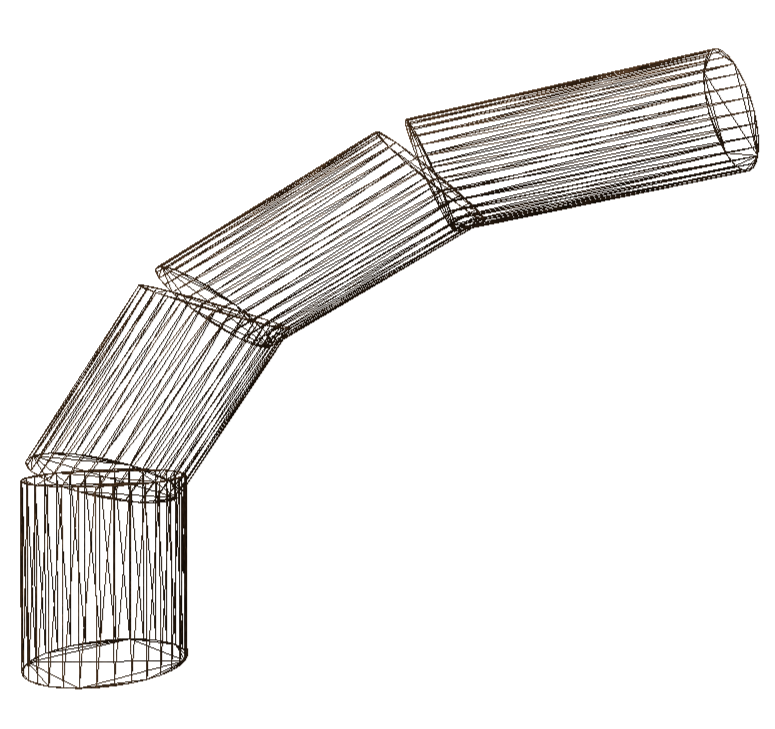
\includegraphics[scale=0.2]{Diagrams/stackedBranchesMesh.png}
		}
		\caption{Example of the continuity problem faced with stacked branching with a 25$^{\circ}$ bend per joint.}
	}
\end{figure}

\FloatBarrier

\noindent
This simple method of stacking cylinders gives a reasonable looking tree structure and it is usually good enough when the angles of branches are not more than 25$^{\circ}$ and the size of the branches do not change. However for a much more convincing tree structure there will need to be a better solution. The logical next step would be to actively link the branch segments together. This requires a number of things to take place, first of all the vertices from the previous branch top must be linked with the new top of the branch. These are the circles of vertices at either end of each branch segment. These circles will have to rotate depending on the bending direction of the branch. This means that the final model will not be made up of a large number of the same model but rather a single model with many linked branches. An example of this can be seen below:

\begin{figure}[htbp]
	{\centering
		\vspace{7px}
		\setlength{\fboxrule}{1pt}
		\fbox{
			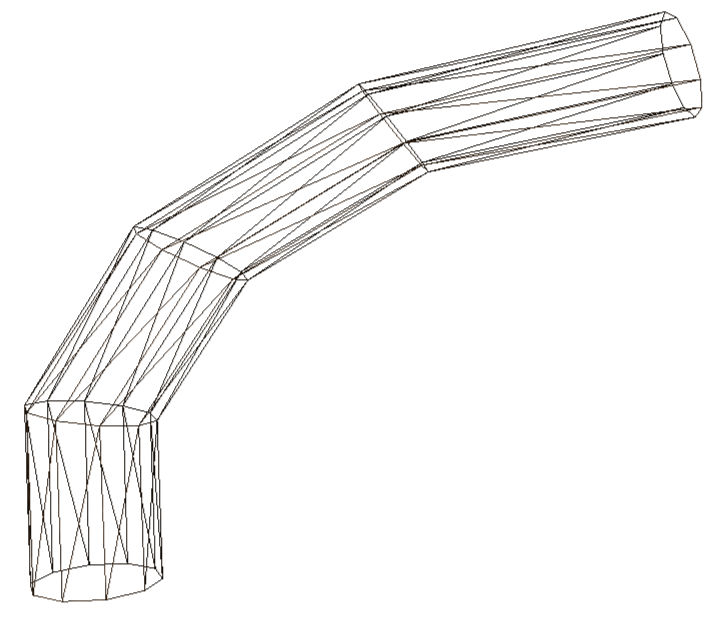
\includegraphics[scale=0.2]{Diagrams/linkedBranchesMesh.png}
		}
		\caption{Example of linked branching with a 25$^{\circ}$ bend per joint.}
	}
\end{figure}
\FloatBarrier

\noindent
This method of branch generation gives a very similar result at first glance to that of stacking cylinders. Although it does have a number of advantages, firstly it completely avoids the branch gap problem that happens with angle changes as well as branch size changes. It also means that the resolution is dynamic, meaning the number of vertices that make up a cylinder can be dynamically changed. This means that a very high resolution tree can be rendered which may look very smooth but will take a lot more computational resources, or a very low resolution tree can be rendered with more jagged edges but will require a lot less computational resources. This can be seen in figure \ref{} below, where similar a looking branch can be acheived using less than half the number of vertices, with joined branches instead of stacked branches.

\begin{figure}[htbp]
	{\centering
		\vspace{7px}
		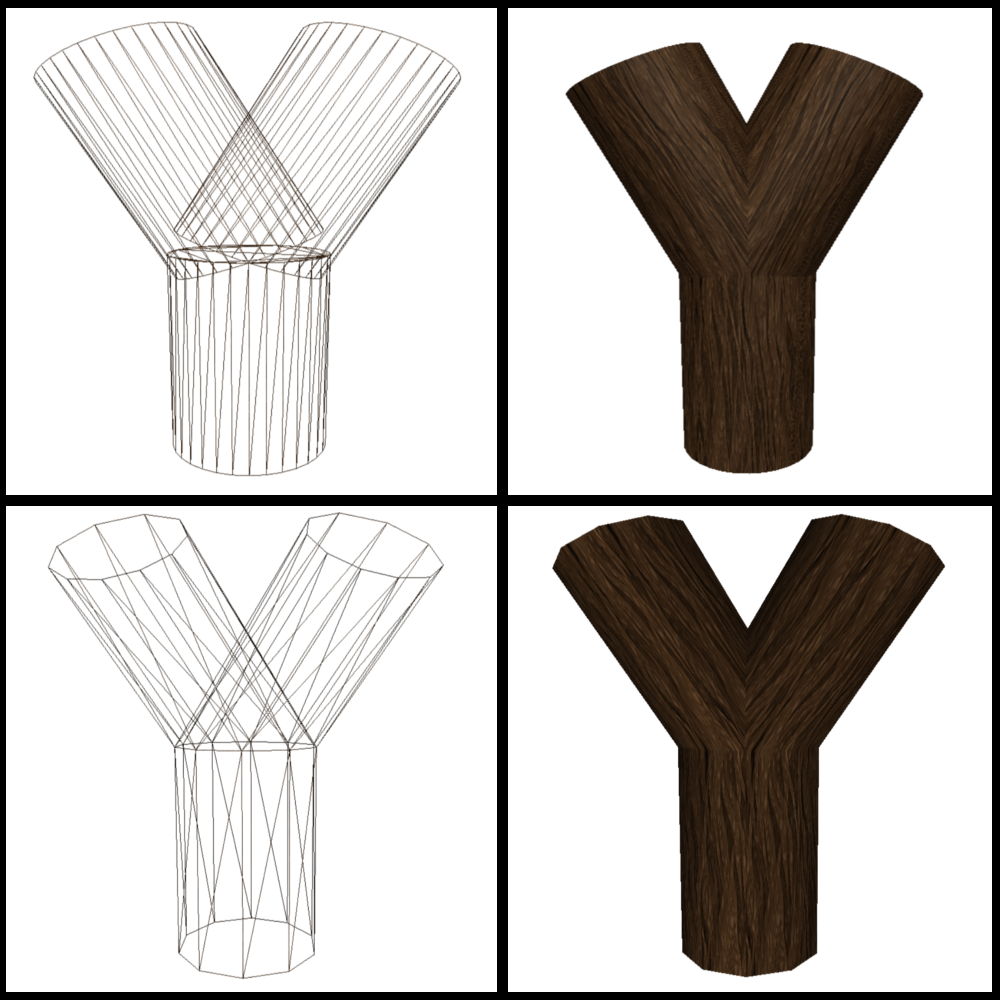
\includegraphics[scale=0.2]{Diagrams/StackedVsLinked.png}
		\caption{Stacked Vs Linked.}
	}
\end{figure}
\FloatBarrier



\section{Renderer}

\noindent
The renderer is the final stage in the procedural generation pipeline. It takes all of the 3D models generated by the model generator, such as leaves, branches and flowers and renders them on the screen.  For this thesis, the \acrlong{opengl} (\acrshort{opengl}) application programming interface is use used to efficiently render the models on the screen using the \acrlong{gpu} (\acrshort{gpu}). 

The \acrshort{gpu} is a specially designed piece of harware for processing computer graphics and image processing, it has hundereds of individual compute cores which can be used in parallel. Due to the highly parallel nature of the \acrshort{gpu}, the \acrshort{opengl} framework helps to abstract the hardware and create an interface to interact with the \acrshort{gpu} in a simpler way. There are a number of other types of graphics \acrshort{api} such as Vulkan, Metal or DirectX. These \acrshort{api}s all provide a way of interacting with the hardware behind the scenes, However, they each have a different approach. Therefore, this section will not be be going into great detail about about the specifics of \acrshort{opengl} but rather the general concepts required for rendering the plant model on the screen.

\subsection{Models and Buffer Objects}

The model generator produces all of the information neccessary for the renderer to produce the result on the screen. In general the model data will consist of vertex data, texture co-ordinates and vertex normals. The vertex data is simply position of a point within a model, three vertices make up a face and the faces are what are ultimately rendered on the screen. The texture co-ordinates are the locations on a texture image which maps directly to the model vertices. Finally the vertex normals simply known as normals are the average normal vector. A normal vector being the vector that is purpendicular to the surface at a given point, and can be used for Phong shading or other types of lighting techniques.  

One of the most important parts of the rendering process is buffering the model data onto the \acrshort{gpu}. The \acrlong{vbo} (\acrshort{vbo}) is a data structure within the \acrshort{opengl} library which can be used to store this data on the \acrshort{gpu}. Generally, the data is stored as a single buffer or array with the first 3 values being a vertex position, the second two being a texture co-ordinate and the last three being a vertex normal. 

\begin{figure}[htbp]
	{\centering
		\vspace{7px}
		\setlength{\fboxrule}{1pt}
		\fbox{
			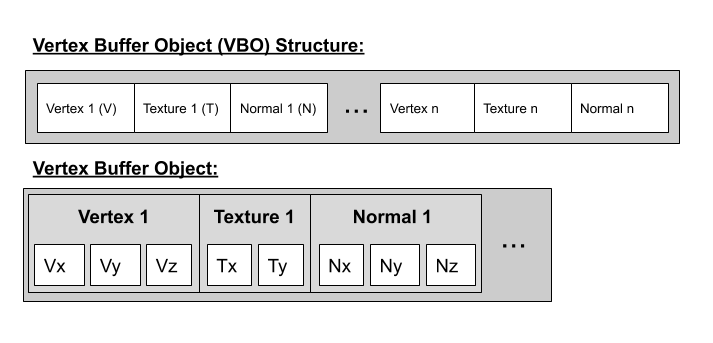
\includegraphics[scale=0.5]{Diagrams/VertexObjects.png}
		}
		\caption{Diagram showing the structure of a vertex buffer object.}
	}
\end{figure}
\FloatBarrier

 










\chapter{String Interpreter Implementation}

\lettrine[lines=3]{T}{}he string interpreter is one of the major components of the L-system, it is the final step in the process of procedural generation. The output of this stage of processing is dependant on what the L-system is representing, in this case it is responsible for interpreting the resulting string of modules, and uses this to generate the 3D models, structures and data of the resulting plant which is then rendered and simulated on the screen using the OpenGL framework. The generation of plant-life has three main stages, the first part is a turtle graphics interpreter which takes the string of modules, these modules are interpreted as a set of instructions, starting from the root of the tree and generates a skeleton made up of branch joints, similar to the techniques used in skeletal rigging in animation \cite{gregory2014game}. The joints within the tree skeleton each represent a branch segment which has some information about the properties of that segment. These segements can be used to generate the vertex, index and other data that make up the 3D models of the plant. These models can finally be passed to the renderer which renders the plant on the screen. The stages of string interpretation can be seen in figure \ref{l-system interpreter} below. 

\begin{figure}[htbp]
	{\centering
		\vspace{7px}
		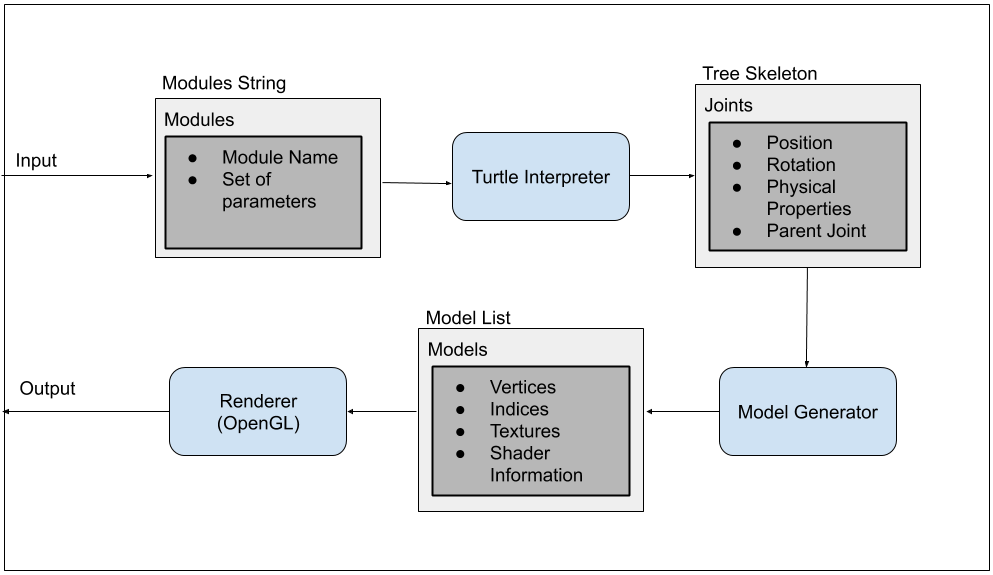
\includegraphics[scale=0.4]{Diagrams/L-systemInterpreter.png}
		\caption{Diagram of the stages of L-system interpretation and rendering} \label{l-system interpreter}
	}
\end{figure}

\noindent
This chapter will outline each stage in the string interpreter implementation for generating 3D models of plant structures as well as well as talking about how the interpreter is able to simulate and animation the plants movements under forces such as gravity and wind in real time. \\

\section{Turtle Graphics Interpreter}


The main job of the turtle graphics interpreter is to take the string of modules from the L-system rewriter and interpret it as a list of turtle graphics instructions. These instructions generate the plants skeleton which is made up of joints, the joints that hold information as to its 3D properties of a particular segement or object. The properties are the position, orientation, physical properties as well as the parent of the joint. The information for each joint is as follows:

\begin{figure}[htbp]
	{\centering
		\vspace{7px}
		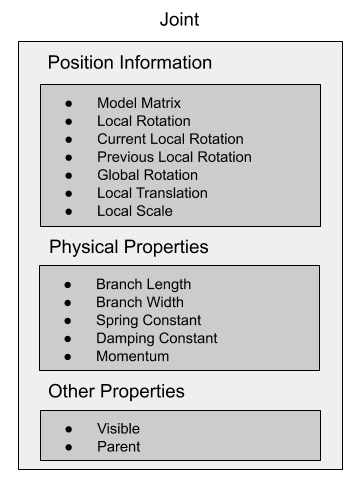
\includegraphics[scale=0.6]{Diagrams/JointDiagram.png}
		\caption{Diagram for the properties of a joint} \label{joint properties}
	}
\end{figure}

\noindent
As you can see from figure \ref{joint properties}, there is large amount of information stored for the position and orientation of each joint. This is because each rotation is stored in both a local and global space. Local space refers to the rotation of the joint relative to the joints parent rotation, this is useful as it allows the manipulation of subsequent child joints but leaving parent joints local rotation unchanged. Global space, also known as world space, is the rotation of the joint relative to the world itself this is useful for understanding the current rotation of the joint relative to the world for instance calculating the torque or force calculations due to gravity. Furthermore it is important to store both the current and previous rotations to calculate the rate of change for physics calculations.

The physical properties for each joint are the parts that will affect the model generation stage as well as the physics simulation. These include the length of the branch stemming from the joint position, the width of the branch, the spring constant or stiffness of the branch, the damping constant for slowing down the branch oscillation and the current momentum of the branch. 

Take the string of modules \say{F(1)[/(90)F(1)$\backslash$ (90)F(1)]-(90)F(1)+(90)F(1)}, the alphabet is made up of seven unique modules F, /, $\backslash$, [, ], + and -. According to the as discussed in previous chapters the \say{F} symbol represents a move forward, and \say{+}, \say{-}, \say{/}, \say{$\backslash$} symbolize different rotations, and the \say{[} and \say{]} represent save and load state respecively. The aforementioned symbols each have a single parameter except the load and save state. It is the turtle graphics interpreters job to understand what these parameters are and how to interpret them. In this case all of the \say{F} modules have the parameter value of 1, and all of the rotation modules have the parameter of 90. These are interpreted as the distance to move forward and the angle to rotate respectively. This interpretation can be represented with the joint structure shown below:

\begin{figure}[htbp]
	{\centering
		\vspace{7px}
		\setlength{\fboxrule}{1pt}
		\fbox{
			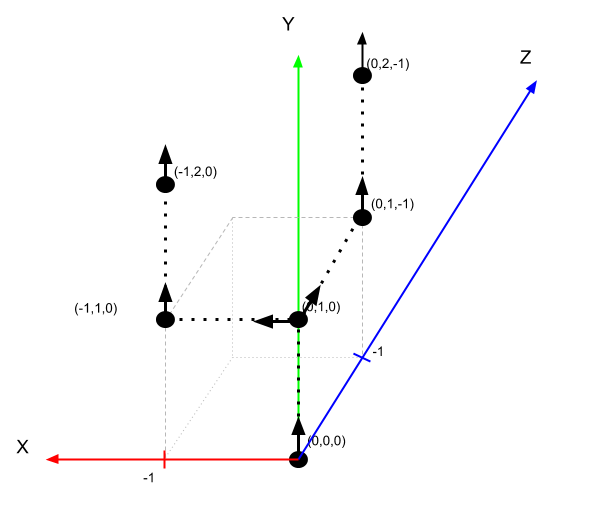
\includegraphics[scale=0.4]{Diagrams/SkeletonJoints.png}
		}
		\caption{Diagram of a simple plant skeleton with joint position and orientation.}
	}
\end{figure}

\FloatBarrier


\section{Model Generator}

\begin{flushleft}

Modeling the branches of a plant is one of the most important parts for the overall look and feel of that plant that is being generated. The L-system described in the previous sections is able to describe the details about the plants structure, for instance the position, width, length, weight and other important information. The job of the model generator is to take this information and intelligently generate the models vertices, normals, texture coordinates and other information that can then be provided to the OpenGL renderer and finally to the GPU to be rendered on the screen. \\

\vspace{5mm}

The simplest way to generate a model for a branching structure of a plant would be to take a number of cylinders, and to rotate and stack them according to each joints position in 3D space. The up side to this approach is that every branch within the plant shares the same object model, depending on the position, rotation and scale of the branch the relavent matrix transforms can be applied. In this way we are able to represent the overall branching structure of the plant. However, there is a problem which is pointed out by Baele and Warz\'{e}e "The branches junction causes a continuity problem: to simply stack up cylinders generates a gap" \cite{baele2005real}. This can be shown in the figure below:

\FloatBarrier

\begin{figure}[htbp]
	{\centering
		\vspace{7px}
		\setlength{\fboxrule}{1pt}
		\fbox{
			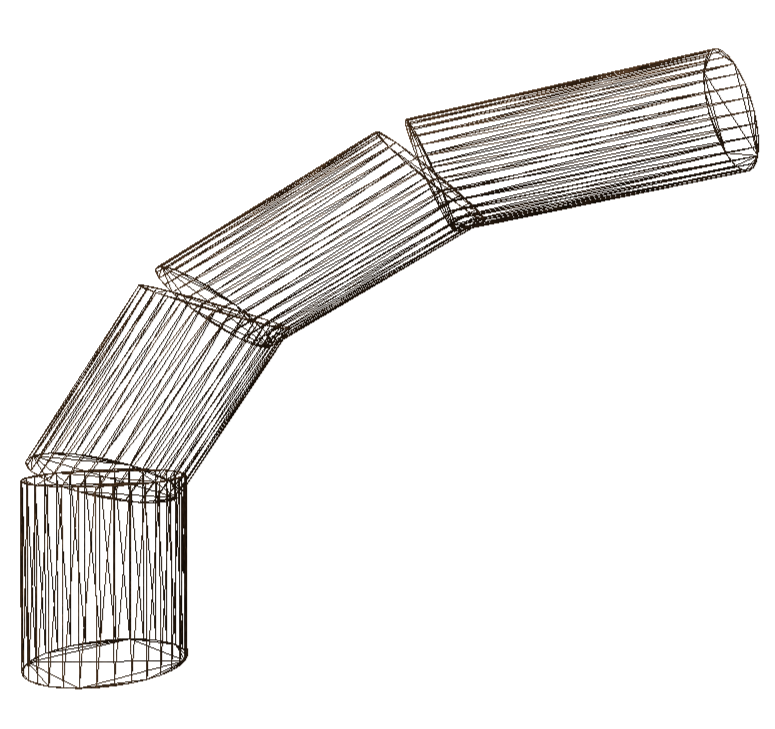
\includegraphics[scale=0.2]{Diagrams/stackedBranchesMesh.png}
		}
		\caption{Example of the continuity problem faced with stacked branching with a 25$^{\circ}$ bend per joint.}
	}
\end{figure}

\FloatBarrier

\vspace{5mm}


\vspace{5mm}

This simple method of stacking cylinders gives a reasonable looking tree structure and it is usually good enough when the angles of branches are not more than about 25$^{\circ}$ and the size of the branches do not change. However for a much more convincing tree structure we will want to do better than this. The logical next step would be to actively link the branch segments together.

\FloatBarrier

\begin{figure}[htbp]
	{\centering
		\vspace{7px}
		\setlength{\fboxrule}{1pt}
		\fbox{
			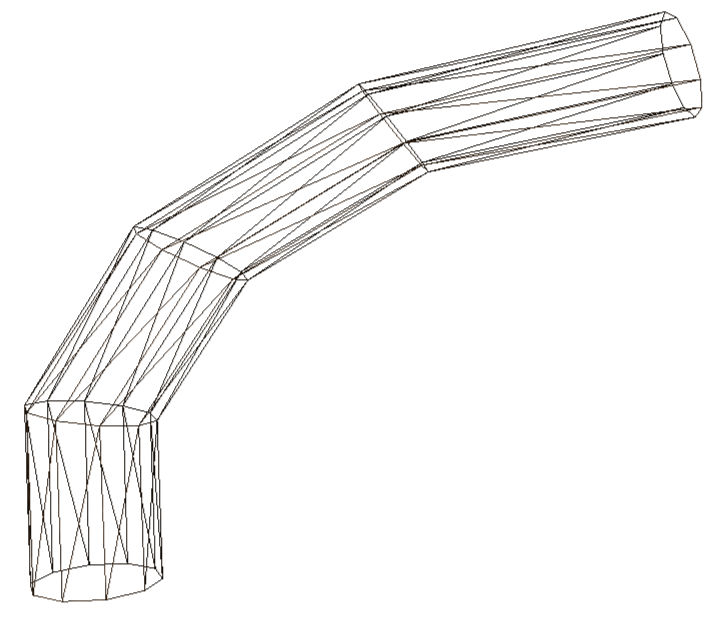
\includegraphics[scale=0.2]{Diagrams/linkedBranchesMesh.png}
		}
		\caption{Example of linked branching with a 25$^{\circ}$ bend per joint.}
	}
\end{figure}

\FloatBarrier

\end{flushleft}

\section{Renderer}

\begin{flushleft}


\end{flushleft}

\section{Displaying the L-system Instructions} \label{Display L-system Instructions}

\subsection{Basic 2D L-systems} 

There are a number of fractal geometry that have become well known particularly with regards to how they can seemingly imitate nature \cite{mandelbrot1982fractal}. Particularly with the geometry such as the Koch snowflake which can be represented using the following L-system.

\begin{figure}[htbp]
	\raggedright
	\textbf{\underline{Koch Curve:}} \\
	\#n = 4; \\
	\#define r 90; \\
	\#w : F(1); \\
	\#p1 : F(x) : * : F(x)+(r)F(x)-(r)F(x)-(r)F(x)+(r)F(x);\\
	{\centering
		\vspace{7px}
		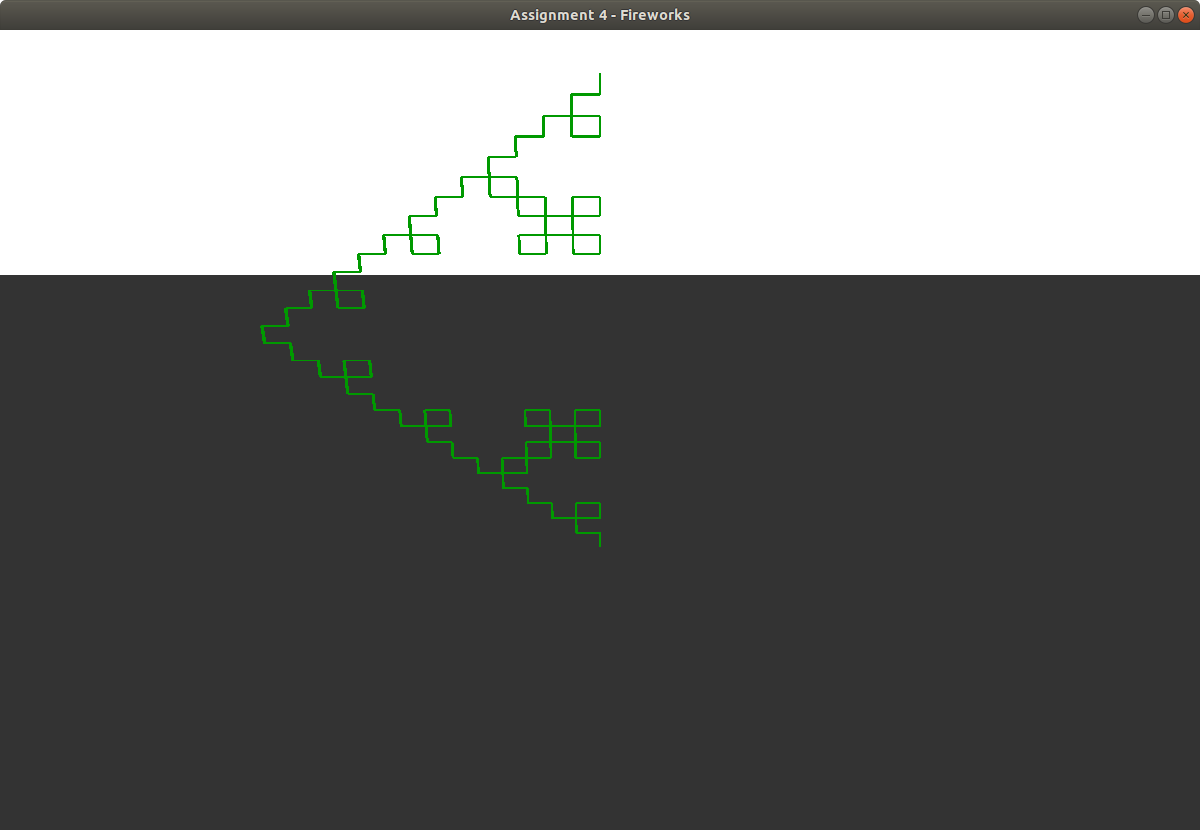
\includegraphics[scale=0.15]{KochCurve/KochCurve04.png}
		\caption{Koch Curve.}
	}
\end{figure}
\begin{figure}[htbp]
	\raggedright
	\textbf{\underline{Sierpinski Triangle:}} \\
	\#n = 4;\\
	\#define r 60;\\
	\#w : F(1);\\
	\#p1 : F(x) : * : X(x)-(r)F(x)-(r)X(x);\\
	\#p2 : X(x) : * : F(x)+(r)X(x)+(r)F(x);\\
	{\centering
		\vspace{7px}
		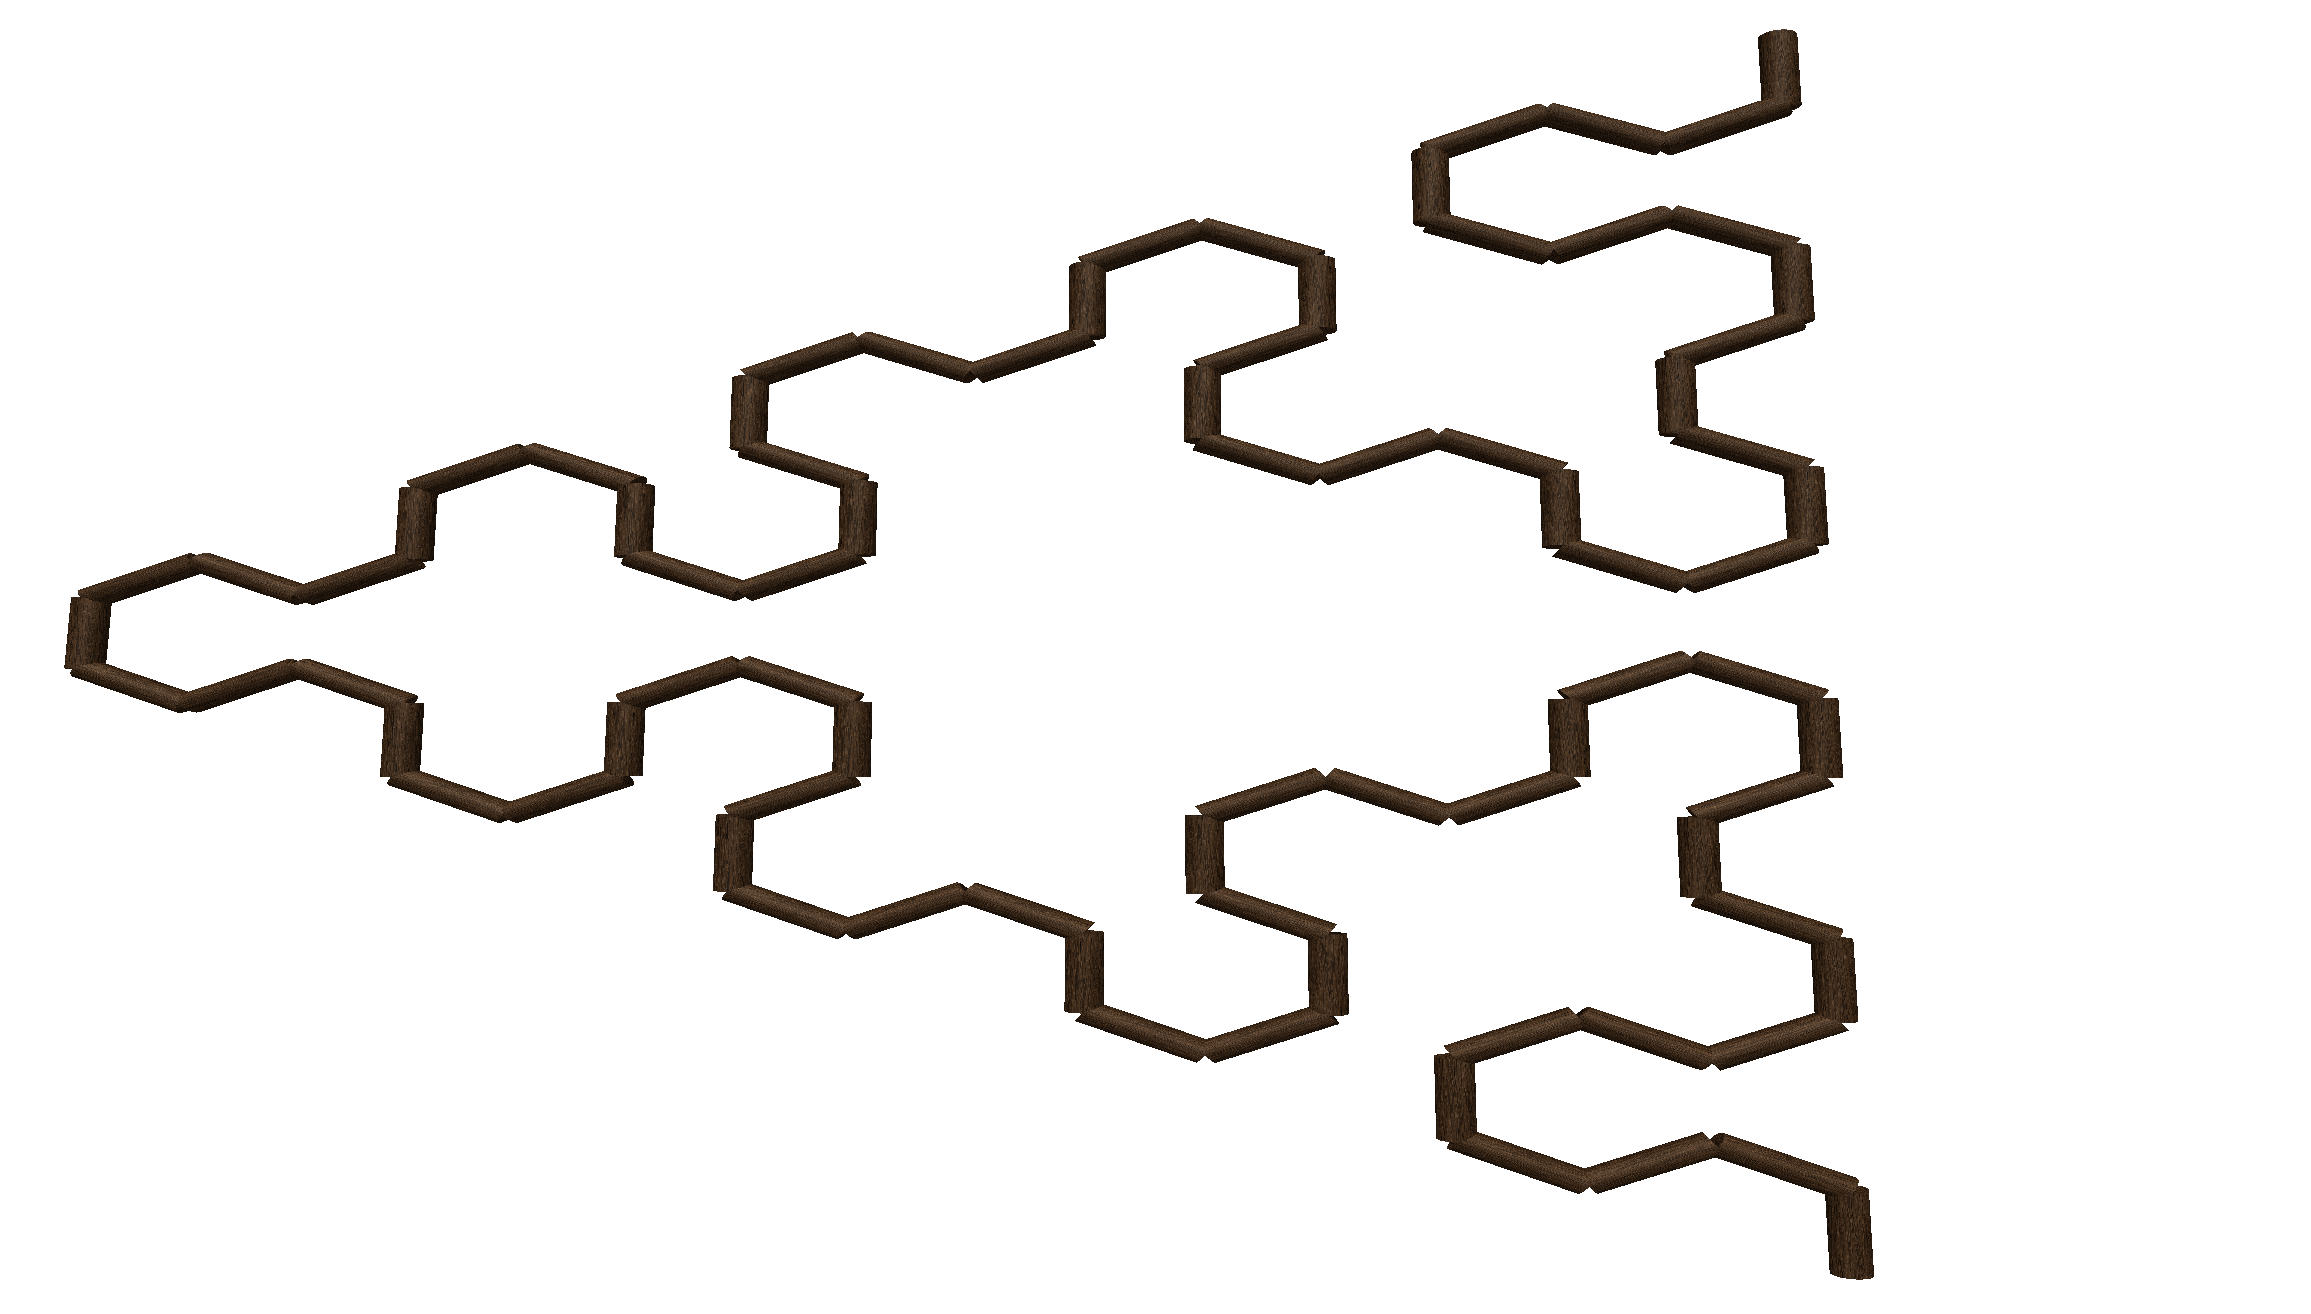
\includegraphics[scale=0.15]{SierpinskiTriangle/SierpinskiTriangle04.png}
		\caption{Sierpinski Triangle.}
	}
\end{figure}
\begin{figure}[htbp]
	\raggedright
	\textbf{\underline{Fractal Plant:}} \\
	\textbf{Alphabet:} X, F\\
	\textbf{Constants:} +, -, [, ] \\
	\textbf{Axiom:} X \\
	\textbf{Angle:} 25$^\circ$ \\
	\textbf{Rules:} \\
	X $\rightarrow$ F-[[X]+X]+F[+FX]-X\\
	F $\rightarrow$ FF \\
	{\centering
		\vspace{7px}
		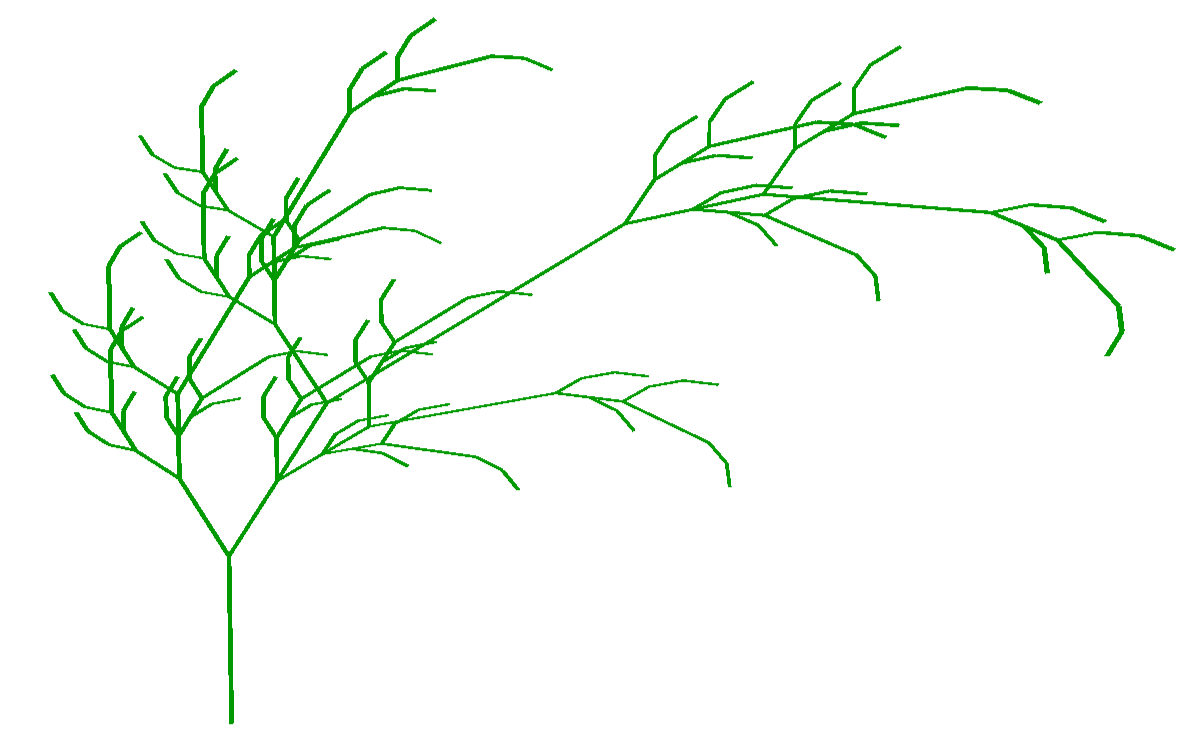
\includegraphics[scale=0.15]{FractalPlant/FractalPlant05.png}
		\caption{Fractal Plant.}
	}
\end{figure}
\begin{figure}[htbp]
	\raggedright
	\textbf{\underline{Fractal Bush:}} \\
	\textbf{Alphabet:} F\\
	\textbf{Constants:} +, -, [, ] \\
	\textbf{Axiom:} F \\
	\textbf{Angle:} 25$^\circ$ \\
	\textbf{Rules:} \\
	F $\rightarrow$ FF+[+F-F-F]-[-F+F+F]\\
	{\centering
		\vspace{7px}
		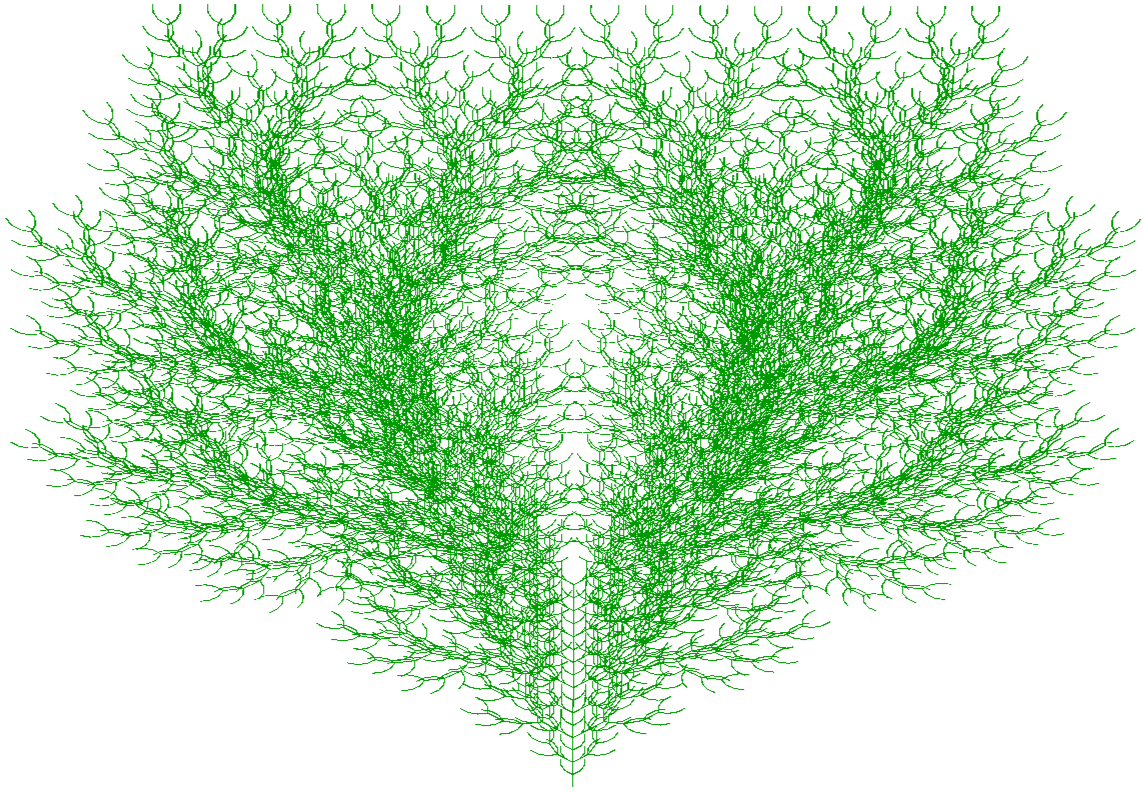
\includegraphics[scale=0.15]{FractalBush/FractalBush06.png}
		\caption{Fractal Bush.}
	}
\end{figure}

\FloatBarrier

\subsection{The Use of L-systems in 3D applications}

\begin{flushleft}

L-systems have been talked about and researched since its inception in 1968 by Aristid Lindenmayer. Over the years it's usefulness in modelling different types of plant life has been very clear, however its presence has been quite absent from any mainstream game engines for the most part, these engines relying either on digital artists skill to develop individual plants or on 3rd party software such as SpeedTree. These types of software use a multitude of different techniques however their methods are heavily rooted in Lindenmayer Systems. 

\end{flushleft}


\chapter{Findings and Data Analysis}
\input{chapters/chapter07}

\chapter{Discussion}
\input{chapters/chapter08}

\chapter{Conclusions}
\input{chapters/chapter09}

\printglossary[type=\acronymtype]
\printglossary

\appendix
\chapter{Appendix}
\section{Appendix 1}

\section{Bibliography}
\bibliography{chapters/ref}
\bibliographystyle{apalike}






\end{document}



